
\chapter{SYSTEM ANAYLYSIS}
\section{Market Survey}
To comprehend the scope and orientation of the system, it’s essential to conduct a market survey of similar systems. Pet adoption systems, each with its unique features and benefits, come in various forms. In Vietnam, however, most organizations in this field operate through social network pages like Facebook and Instagram, rather than standalone software systems. Notably, the only pet adoption system that stands out from the rest is Hanoi Pet Adoption, which warrants further analysis and evaluation.

\subsection{Overview}
\subsubsection*{Hanoi Pet Adoption}
To comprehend the scope and orientation of the system, it’s essential to conduct a market survey of similar systems. We decided to choose the three below websites as our main targets for analysis and evaluation:
\textbf{Hanoi Pet Adoption}, \textbf{PetRescue}, and \textbf{PetFinder}, each representing Vietnam, Australia, and the United States.

HPA has the following main features:
\begin{itemize}
  \item \textit{Pet profiles:} The system showcases profiles of animals ready for adoption. These profiles include details such as photos, names, genders, ages, colors, and sterilization statuses.
  \item \textit{Dual languages support:} The site has both English and Vietnamese languages available.
  \item \textit{Blogs:}  The system provides blogs about training tips, news, pet health care,...
\end{itemize}

\subsubsection*{PetRescue}

Based in Australia, PetRescue is a widely recognized non-profit organization dedicated to finding homes for rescued pets. The platform connects thousands of rescue groups, shelters, and pounds across Australia, offering a central repository for adoptable animals.

PetRescue's key features include:

\begin{itemize}
  \item \textit{Comprehensive Pet Listings}: The platform provides detailed profiles for each animal, including photos, descriptions, ages, breeds, and health statuses.
  \item \textit{Adoption Stories}: PetRescue features success stories of adopted animals, which helps to promote adoption and provide reassurance to potential adopters.
  \item \textit{Educational Resources}: The site offers extensive resources on pet care, behavior, and training, helping new pet owners to integrate their pets into their homes successfully.
  \item \textit{Support for Rescue Organizations}: PetRescue supports rescue groups by offering them tools to manage their pet listings and connect with potential adopters, enhancing their ability to find homes for rescued animals.
\end{itemize}


\subsubsection*{PetFinder}

PetFinder, a prominent online resource in the United States, is dedicated to promoting pet adoption by connecting potential adopters with a vast network of animal shelters and rescue organizations. The platform's goal is to reduce the number of homeless pets and to advocate for responsible pet ownership.

Here are some of PetFinder's key features:

\begin{itemize}
  \item \textit{Extensive Pet Database}: PetFinder hosts an extensive database of adoptable pets, featuring detailed profiles with photos, descriptions, breed information, and adoption requirements.
  \item \textit{Mobile Application}: The platform offers a mobile app, allowing users to browse and inquire about adoptable pets on-the-go.
  \item \textit{Adoption Resources}: PetFinder provides a wealth of information on the adoption process, pet care tips, and training advice.
  \item \textit{Shelter and Rescue Support}: PetFinder offers tools and resources for shelters and rescue groups to manage their listings and reach a broader audience, increasing their chances of finding homes for their animals.
\end{itemize}

By analyzing these systems, we gain valuable insights into the functionalities, strengths, and areas for improvement that can guide the development of our own platform, ensuring it meets the needs of both the animals and the adopters effectively.

\subsection{Evaluation}
\subsubsection*{Hanoi Pet Adoption}

HPA provides a comprehensive and effective pet adoption support process. However, its limitation lies in its exclusivity - only system administrators of the organization are permitted to post pet profiles onto the system.

Currently, the system requires manual input for posting, filtering, and searching functions. This can pose challenges for individual users, potentially reducing the efficiency of posting and searching, and negatively impacting the user experience.

Lastly, a significant feature that is absent in the system is a notification system. Such a system would alert users when pets that meet their criteria are posted, ensuring that users are promptly informed about potential matches. This feature could greatly enhance the user experience and effectiveness of the pet adoption process.

\subsubsection*{PetFinder}

With extensive database and mobile app, PetFinder provides a highly accessible and efficient platform for pet adoption. The detailed pet profiles and extensive adoption resources help users make informed decisions. The mobile application adds convenience, allowing users to browse adoptable pets on the go. However, PetFinder encounters a crucial problem which is the long loading time, it took over 10-15 seconds to load the application. This problem may severely affect the user experience.

\subsubsection*{PetRescue}

PetRescue may be the one closest to perfection in terms of pet adoption application. Its extensive pet listings and success stories not only promote pet adoption but also build trust and engagement with users. The educational resources and support for rescue organizations further enhance their effectiveness. The only downside of this application is that it has been around for a long time so the UI/UX is quite outdated.


\subsection{Improvements and Adaptions}

After a thorough review of the strengths and weaknesses of existing systems, we have identified several potential enhancements that could significantly improve the user experience and functionality of the system.

Firstly, we propose to \textbf{expand the HPA system}. Currently, the pets are only posted by system administrators. However, SGT aims to allow individuals wishing to surrender their pets to proactively post about their pets for adoption. This expansion would not only increase the number of pets available for adoption but also provide a platform for pet owners and organizations to share valuable information and updates about their pets.

Secondly, we suggest the implementation of \textbf{interactive pet profiles} with user friendly UI/UX. This feature would allow users to visit and interact with pet profiles and posts. This interaction could include liking, commenting, or sharing a pet’s profile.

Next, we recommend \textbf{applying Artificial Intelligence (AI) technology to enhance the posting and searching} functionality of the system. With this feature, users could simply upload a pet image, and the AI would automatically populate most of the input fields, such as breed, and color. This would not only simplify the process of posting a pet profile but also increase the accuracy and consistency of the pet information in the system.

In addition, we also want to adapt the \textbf{management tools for organizations} like PetRescue and PetFinder, offering tools and resources for rescue groups to manage their pet listings and interact with potential adopters will streamline the adoption process and support the efforts of these organizations.

Lastly, we propose the implementation of a \textbf{notification system}. This system would alert users when a pet that matches their preferences becomes available on the system. User criteria for filtering pet profiles (such as breed, age, or size) will be referenced, and then users can receive notifications when a matching pet is posted. This would ensure that users don’t miss out on potential matches and can act quickly to adopt their desired pet.

In conclusion, these enhancements aim to make the system more user-friendly, efficient, and effective in connecting pets with potential adopters. We believe that by implementing these changes, we can take a significant step toward our goal of finding a loving and suitable home for every pet.

\section{Stakeholders}
Stakeholders for a project focused on creating a pet adoption platform in Vietnam would include a diverse range of individuals, organizations, and groups with an interest in or influence over the project. Here are some key stakeholders:
\begin{itemize}
  \item \textit{Administrator:} The administrator is responsible for managing and overseeing the platform's operations. They have control over user accounts, content moderation, and the overall functionality of the website.
  \item \textit{Pet Adopter:} Pet adopters are individuals looking to provide a loving home to pets available for adoption. They may already own pets or be first-time pet owners. Pet adopters interact with pet owners and adoption agencies through messaging and inquiries about available pets. They can also share their adoption stories and experiences with the platform's community.
  \item \textit{Pet Owner:} Pet owners are individuals who currently own and care for pets, including dogs, cats, or other animals. Or those, for various reasons, have decided to give their pets to new homes. Reasons may include relocation, financial constraints, allergies, or changes in life circumstances.
  \item \textit{Guest:} Guests are individuals who visit the platform without creating an account or logging in. They have limited access to platform features and content. Guests can browse public content, view pet listings, read provided blogs, and explore the platform's resources. They can also choose to create an account to access more features.
  \item \textit{Pet Adoption Agencies and Shelters:} Organizations involved in pet adoption, rescue, and rehoming would benefit from the platform as it could help them find suitable homes for abandoned or rescued animals. They might also contribute content and listings.
  \item \textit{Pet-Related Businesses:} Pet stores, pet food suppliers, grooming salons, veterinary clinics, and other businesses in the pet industry have a stake in the project. They could use the platform to advertise their products and services to a targeted audience.
  \item \textit{Veterinarians:} Veterinarians play a crucial role in pet healthcare. They might use the platform to provide information, answer questions, and offer telehealth services. Their expertise can be valuable to pet owners.
  \item \textit{Investors and Funders:} Individuals or organizations providing funding or investment for the development and scaling of the platform are stakeholders with a financial interest.
\end{itemize}

Understanding and engaging with these stakeholders will be important for the success and sustainability of the project. Each stakeholder group may have different needs, interests, and concerns that should be addressed during the project's planning and execution.

\section{Requirements eliciation}

\subsection{Functional Requirements}

\begin{longtblr}[
    caption = {Functional Requirements},
    label = {tblr:func_req},
  ]{
    vline{1-3} = {-}{},
    hline{-} = {1-2}{},
    colspec={X[2,l] X[5, l]},
  }
  \textbf{Group}                                & \textbf{Requirements}                                                                                                                                                                                                                                                                                                                                                                                                                                                                                                                                                                      &  &  \\
  \textbf{Authentication and authorization}     & {
    -~~~~~~~
    Users can create new accounts by providing personal information.
    \\-~~~~~~~
    Users can log into the system using Google accounts.
    \\-~~~~~~~
    Users can log into the system by
    providing a registered email and password.
    \\-~~~~~~~
    Users can send applications to the system to update their accounts to
    Organization accounts.
    \\-~~~~~~~
    Admins can verify Organizations’ registration and upgrade users’
    accounts.
    \\-~~~~~~~
    Users can reset or recover their account passwords.
    }                                                          &  &  \\
  \textbf{Pet profile management}               & {
    -~~~~~~~
    Users can create pet profiles by giving details such as name, species,
    breed, age, color, health status, sterilization status, pictures, and videos
    of pets.
    \\-~~~~~~~
    Users can provide information about breed, species, and color by
    uploading pets’ pictures.
    \\-~~~~~~~
    Pet photos and text inputs must be sensitive-validated before
    uploading.
    \\-~~~~~~~
    Users can edit their pet profiles.
    \\-~~~~~~~
    Users can publish, hide, or remove their pet profiles.
    \\-~~~~~~~
    Admins can remove or hide any pet profiles of the system.
    } &  &  \\
  \textbf{Pet profile filter and view}          & {
    -~~~~~~~
    Users can search for pets by providing filtering options such as name,
    species, breed, age, color, health status, and sterilization status.
    \\-~~~~~~~
    Users can search for pets by providing pets’ pictures.
    \\-~~~~~~~
    Users can view pet profiles with detailed information such as name,
    species, breed, age, color, health status, sterilization status, pictures,
    and videos of pets
    }                                                                                                                                                                &  &  \\
  \textbf{Pet adoption}                         & {
    -~~~~~~~
    Users can submit applications to adopt pets on the system.
    \\-~~~~~~~
    Users can view, decline, or accept adoption applications sent to their
    pets.
    }                                                                                                                                                                                                                                                                                                                                                                                                                &  &  \\
  \textbf{User interaction and engagement}      & {-~~~~~~~
  Pet
  Adopters can send messages to Pet Owners, Organizations, and Admins.
  \\-~~~~~~~PetAdopters have to update their pets’ status every seven days[1]~ from the date they received the petsby uploading posts in the adopt status section of the pet profile.\\-~~~~~~~
  Pet
  Adopters can set their posts public for all users or just Admins, and Pet
  Owners.
  \\-~~~~~~~
  Admins
  and Pet Owners can view and interact with posts from Pet Adopters.
  \\-~ ~ ~ ~ All users of the system can view and interact
  with posts from Pet Adopters if the posts are public.~ ~ ~~}        &  &  \\
  \textbf{Blog management}                      & {
    -~~~~~~~
    Admins and Organizations can create and publish blogs.
    \\-~~~~~~~
    Organizations can apply advertisements on their blogs.
    \\-~~~~~~~
    Organizations can edit or remove their blogs.
    \\-~~~~~~~
    Admins can hide or remove any blogs of the system.
    }                                                                                                                                                                                                                                                                                                             &  &  \\
  \textbf{Advertisement and payment}            & {
    -~~~~~~~
    Organizations can choose advertisement duration with different prices.
    \\-~~~~~~~
    Organizations can pay advertisement fees through an online banking
    service.
    \\-~~~~~~~
    Admins can receive advertisement fees through an online banking
    service.
    \\-~~~~~~~
    System provides admins and organizations information like payment
    status and invoices.
    }                                                                                                                                                                                                   &  &  \\
  \textbf{Notifications}                        & {
    -~~~~~~~
    Users can receive notifications on new pet adoption applications.
    \\-~~~~~~~
    Users can receive notifications on new pets’ status posts uploaded.
    \\-~~~~~~~
    Users can receive notifications on new pet profiles matching their
    criteria.
    }                                                                                                                                                                                                                                                                                                                      &  &  \\
  \textbf{System statistics for administrators} & -~~~~~~~
    Admins can get statistics about systems usages, such as the number of
    pet profiles, adopted pets; number of users and Organizations; number of
    blogs, and the total amount of advertisement fee.                                                                                                                                                                                                                                                                                                                                                                            &  &  
\end{longtblr}


\subsection{Non-Functional Requirements}

\begin{longtblr}[
    caption = {Non-Functional Requirements},
    label = {tblr:non_func_req},
  ]{
    vline{1-3} = {-}{},
    hline{-} = {1-2}{},
    colspec={X[2,l] X[5, l]},
  }
  \textbf{Group} & \textbf{Requirements} \\
  \textbf{Performance} & {
    -~~~~~~~
    The system should respond to pages loading in under 2 seconds.
    \\-~~~~~~~
    The period for payment transaction (from starting the transaction to receiving the result notification) period is at most 10 seconds.
    \\-~~~~~~~
    The period for pet profiles filtering is at most 2 seconds.
    \\-~~~~~~~
    The delay time for real-time messages is at most 0.5 seconds.
  } \\
  \textbf{Localization} & {
    -~~~~~~~
    All the system data and user inputs of time are in the format of "dd/mm/yyyy”.
    \\-~~~~~~~
    All the system data and user inputs of address are in the format of “street, ward, district, city”.
    \\-~~~~~~~
    The language used in the system is Vietnamese.
  } \\
  \textbf{Security} & {
    -~~~~~~~
    The system data (such as email, password, and personal information) must be encrypted before being stored in the database.
    \\-~~~~~~~
    User unauthorized access to system features and data must be prevented using authorization with JWT tokens.
    \\-~~~~~~~
    System uses secured data transmission over the internet (TLS, HTTPS).
    \\-~~~~~~~
    System components (API servers, database servers, file storage,..) must be protected from external accesses.
    \\-~~~~~~~
    System must have at least one backup database that is kept synchronized for potential problems with the main database.
    \\-~~~~~~~
    User register requests must be challenged by a reCAPTCHA service.
  } \\
  \textbf{Compatibility} & {
    -~~~~~~~
    The web application of the system functions correctly on popular web browsers, such as Chrome, Firefox, Safari, and Edge.
    \\-~~~~~~~
    The web application of the system supports responsiveness and works well on various devices and screen sizes (smartphones, tablets, desktops).
  } \\
  \textbf{Reliability} & {
    -~~~~~~~
    The system must perform without failure in 95 percent of use cases during a month.
    \\-~~~~~~~
    Run smoothly when 1000 users access at the same time.
  } \\
  \textbf{Usability} & {
    -~~~~~~~
    The maximum amount of time for new users to get familiar with the web application of the system is 15 minutes.
    \\-~~~~~~~
    The steps to give and adopt a pet must be short and straightforward.
  } \\
  \textbf{Scalability} & {
    -~~~~~~~
    The backend components of the system can be reused to build a mobile application in the future.
    \\-~~~~~~~
    The system supports horizontal scaling to add more servers to accommodate increased user activity.
    \\-~~~~~~~
    The design patterns of the systems must be able to further implement new features in the future.
  } \\
\end{longtblr}


\section{Use-case analysis}
\subsection{The whole system}

\textit{Figure 2.1} serves as a foundational element in our analysis, offering a high-level depiction of the primary actors and their associated functionalities within the adoption application system.

\begin{figure}[H]
  \centering
  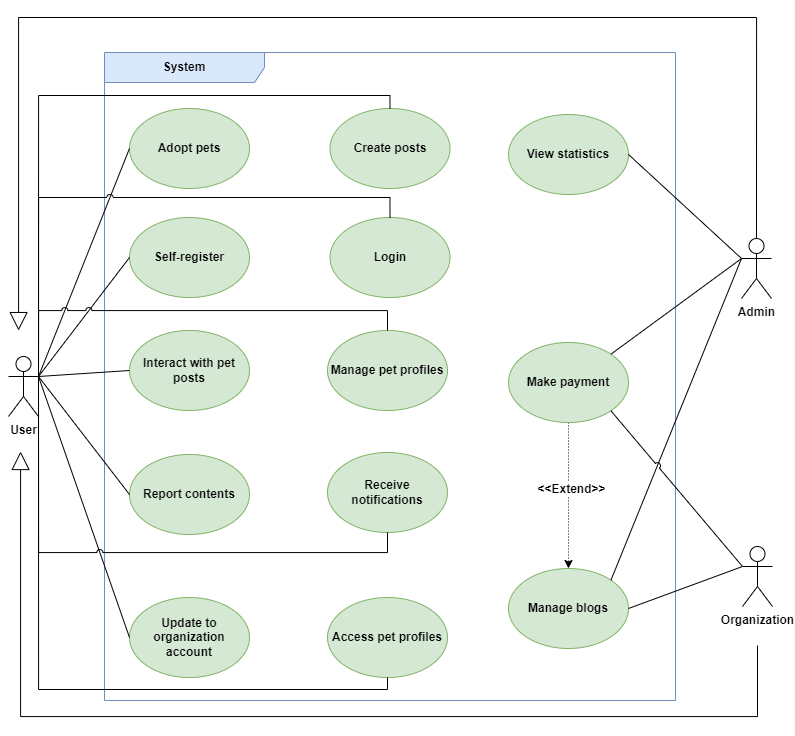
\includegraphics[width=0.6\textwidth]{Figures/system_ucd.png}
  \caption{Use-case diagram of the whole system}
  \label{fig:whole-system_activity_diagram}
\end{figure}

The comprehensive view Figure 1 provided sets the stage for a detailed exploration of each actor's specific use cases, providing a comprehensive understanding of the system's functionalities. As we proceed with our analysis, we will delve into the intricate details of each key function, exploring their roles and contributions to the overall functionality of the adoption application system.

\subsection{Login}

\begin{figure}[H]
  \centering
  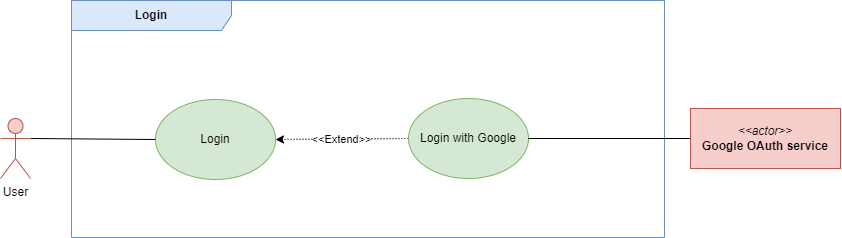
\includegraphics[width=0.7\textwidth]{Figures/login_ucd.png}
  \caption{Use-case diagram of the login function}
  \label{fig:login_activity_diagram}
\end{figure}

\begin{longtblr}[
    caption = {Use Case: Log In},
    label = {tblr:login_use_case},
  ]{
    vline{1-16} = {-}{},
    hline{-} = {1-2}{},
    colspec={X[3,l] X[7, l]},
  }
  \textbf{Use-case name} & \textbf{Log in} \\
  \textbf{Actors} & {
    User, Google OAuth Service
  } \\
  \textbf{Preconditions} & {
    User at login page
  } \\
  \textbf{Postconditions} & {
    Users log in successfully and can access authorized features.
  } \\
  \textbf{Triggers} & {
    1. Users access any authorized features of the system without being authorized.
    \\2. Users want to log in to the system.
  } \\
  \textbf{Normal flow} & {
    1. Users click on the login button of the system. The system displays a login form screen.
    \\2. User provides authentication information including email and password.
    \\3. The system verifies the authentication information.
    \\4. System grants access permission to users.
  } \\
  \textbf{Alternative flows} & {
    Alternative flow 1, at step 1:
    \\1. Users access any authorized features of the system without being authorized.
    \\Alternative flow 2:
    \\1. Users choose the option of login with a Google account. The system displays a Google login form screen.
    \\2. Users provide Google authentication information.
    \\3. Google Auth service verifies the authentication information and generates access tokens.
    \\4. System validates access token and grants access permission to users.
  } \\
  \textbf{Exceptions} & {
    1. Users input the wrong authentication information.
    \\2. Users do not have an account.
    \\3. Users do not have a Google account.
    \\4. Google OAuth Service works incorrectly.
  } \\
\end{longtblr}


\subsection{Register}

\begin{longtblr}[
    caption = {Use Case: Register},
    label = {tblr:register_use_case},
  ]{
    vline{1-13} = {-}{},
    hline{-} = {1-2}{},
    colspec={X[3,l] X[7, l]},
  }
  \textbf{Use-case name} & \textbf{Register} \\
  \textbf{Actors} & {
    User
  } \\
  \textbf{Preconditions} & {
    Users at register page
  } \\
  \textbf{Postconditions} & {
    Users register new accounts successfully
  } \\
  \textbf{Triggers} & {
    Users want to create new accounts and can access authorized features
  } \\
  \textbf{Normal flow} & {
    1. Users click on the register button of the system. The system displays a register form screen.
    \\2. Users provide authentication information (including email and password) and other personal information.
    \\3. The system verifies register information and sends validation emails to users.
    \\4. Users click on the link in the validation emails. The system creates new accounts and grants access permission to the guests (now become users).
  } \\
  \textbf{Alternative flows} & {
    Alternative flow 1, from step 3:
    \\3. System verifies provided information as invalid and rejects the registration.
  } \\
  \textbf{Exceptions} & {
    1. Provided emails are already in use.
    \\2. Guests do not confirm the validation email on time.
  } \\
\end{longtblr}


\subsection{Update to organization account}

\begin{figure}[H]
  \centering
  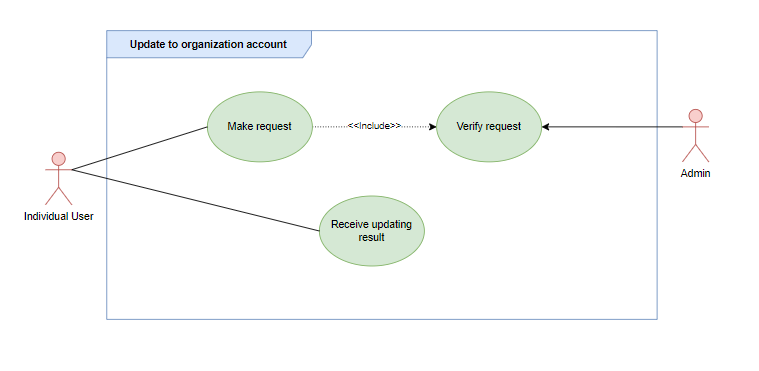
\includegraphics[width=0.7\textwidth]{Figures/update_org_ucd.png}
  \caption{Use-case diagram of the update to organization account function}
  \label{fig:update-org_activity_diagram}
\end{figure}

\begin{longtblr}[
    caption = {Use Case: Update To Organization Account},
    label = {tblr:update_organization_use_case},
  ]{
    vline{1-11} = {-}{},
    hline{-} = {1-2}{},
    colspec={X[3,l] X[7, l]},
  }
  \textbf{Use-case name}     & \textbf{Update to organization account} \\
  \textbf{Actors}            & {
      User, Admin.
  }                                                                    \\
  \textbf{Preconditions}     & {
      1. Admins have logged into the system.
  \\2. Users have an individual user account.
  }                                                                    \\
  \textbf{Postconditions}    & {
      Users update their account successfully.
  }                                                                    \\
  \textbf{Triggers}          & {
      1. Users logged into the systems.
  \\2. Users are on the user profile page.

  }                                                                    \\
  \textbf{Normal flow}       & {
      1. Users choose to update to organization accounts.
  \\2. Users provide some information for verification and submit them.
  \\3. Admins verify the update-account application.
  \\4. The system updates the accounts and notifies the user of the results.
  }                                                                    \\
  \textbf{Alternative flows} & {
      Alternative flow, from step 3:
  \\3. Admins decline the update applications.
  \\4. The system notifies the user of the results.
  }                                                                    \\
  \textbf{Exceptions}        & {

  }                                                                    \\
\end{longtblr}


\subsection{Mange pet profile}

\begin {figure}[H]
\centering
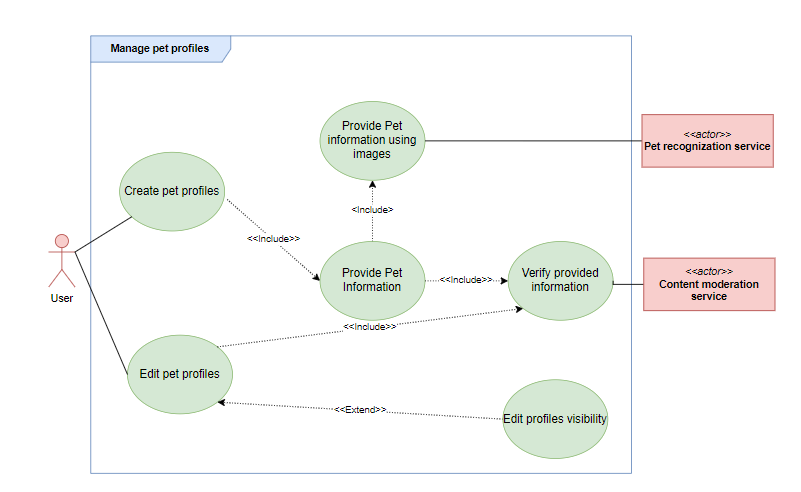
\includegraphics[width=0.7\textwidth]{Figures/manage_pet_ucd.png}
\caption{Use-case diagram of the manage pet profile function}
\label{fig:manage-pet-activity-diagram}
\end{figure}

\begin{longtblr}[
    caption = {Use Case: Manage Pet Profile},
    label = {tblr:manage_pet_profile_use_case},
  ]{
    vline{1-14} = {-}{},
    hline{-} = {1-2}{},
    colspec={X[3,l] X[7, l]},
  }
  \textbf{Use-case name}     & \textbf{Manage pet profile} \\
  \textbf{Actors}            & {
      User, Pet Recognization Service.
  }                                                        \\
  \textbf{Preconditions}     & {
      Users logged successfully into the system.
  }                                                        \\
  \textbf{Postconditions}    & {
      Users create and edit their pet profiles successfully.
  }                                                        \\
  \textbf{Triggers}          & {
      Users access the pet profile management section of the system.
  }                                                        \\
  \textbf{Normal flow}       & {
      1. Users click on the add profiles button of the system. The system displays a form screen of a pet profile.
  \\2. Users input their pet images. Pet Recognition Service automatically fills breed and color fields.
  \\3. Users fill in the remaining fields and submit.
  \\4. The system verifies submitted information using the Content Moderation service.
  \\5. The system creates new pet profiles and notifies the users.
  }                                                        \\
  \textbf{Alternative flows} & {
      Alternative flow 1, from step 2 to step 3:
  \\2. Users input the forms manually.
  \\Alternative flow 2, at step 3:
  \\3. Users edit input fields generated by Pet Recognization Service and submit.
  \\Alternative flow 3:
  \\1. Users choose their available pet profiles and click on the edit button. The system displays a form screen of pet profiles.
  \\2. Users edit and submit their pet information.
  \\3. The system updates the pet profiles and notifies the users.
  \\Alternative of flow 3, from step 2 of alternative flow 2:
  \\2. Users choose to remove their pet profiles. The system asks for confirmation.
  \\3. Users confirm removing pet profiles. The system deletes pet profiles and notifies users.
  }                                                        \\
  \textbf{Exceptions}        & {
      Pet Recognization Service cannot detect and fill in pet information.
  }                                                        \\
\end{longtblr}


\subsection{Access pet profile}

\begin {figure}[H]
\centering
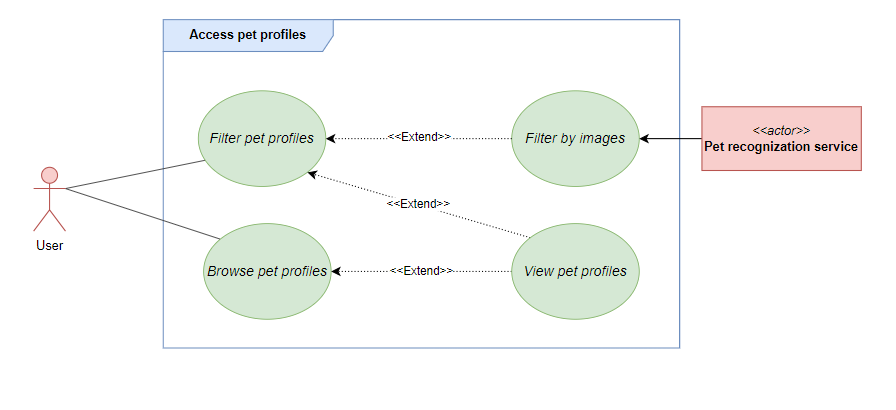
\includegraphics[width=0.7\textwidth]{Figures/access_pet_ucd.png}
\caption{Use-case diagram of the access pet profile function}
\label{fig:access-pet-activity-diagram}
\end{figure}

\begin{longtblr}[
    caption = {Use Case: Access Pet Profiles},
    label = {tblr:access_pet_profiles_use_case},
  ]{
    vline{1-11} = {-}{},
    hline{-} = {1-2}{},
    colspec={X[3,l] X[7, l]},
  }
  \textbf{Use-case name}     & \textbf{Access pet profiles} \\
  \textbf{Actors}            & {
      User
  }                                                         \\
  \textbf{Preconditions}     & {
      User at search page.
  }                                                         \\
  \textbf{Postconditions}    & {
      Users view their desired pets.
  }                                                         \\
  \textbf{Triggers}          & {
      Users access the system and want to find pets.
  }                                                         \\
  \textbf{Normal flow}       & {
      1. Users access the pet section. The system displays the pet section screen.
  \\2. Users select categories to filter. System filter and display list of pets.
  \\3. Users choose a pet profile. The system shows the pet profile details.
  }                                                         \\
  \textbf{Alternative flows} & {
      Alternative flow 1, from step 2:
  \\2. Users select a pet profile displayed in the pet section. The system shows the pet profile details.
  \\Alternative flow 2, from step 3:
  \\3. Users choose to filter by an image. The system sends the image to the pet recognition service.
  \\4. The service extracts information from images. System filter and display list of pets.
  \\5. Users choose a pet profile. The system shows the pet profile details.
  \\Alternative flow 3, at step 2
  \\2. Users filter pets by inputting text keywords.
  }                                                         \\
  \textbf{Exceptions}        & {
      1. The system does not have the user’s desired pet.
  \\2. The pet recognition service cannot extract information from the provided image.
  }                                                         \\
\end{longtblr}


\subsection{Adopt pets}

\begin {figure}[H]
\centering
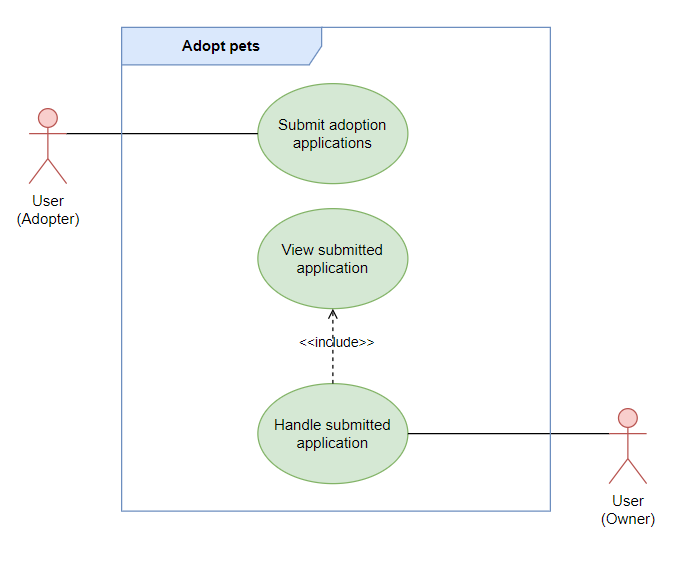
\includegraphics[width=0.7\textwidth]{Figures/adopt_pet_ucd.png}
\caption{Use-case diagram of the adopt pets function}
\label{fig:adopt-pet-activity-diagram}
\end{figure}

\begin{longtblr}[
    caption = {Use Case: Adopt pets},
    label = {tblr:adopt_pets_use_case},
  ]{
    vline{1-12} = {-}{},
    hline{-} = {1-2}{},
    colspec={X[3,l] X[7, l]},
  }
  \textbf{Use-case name} & \textbf{Adopt pets} \\
  \textbf{Actors} & {
    General User
  } \\
  \textbf{Preconditions} & {
    1. Users logged successfully into the system.
    \\2. Pet Adopters find pet profiles successfully.
  } \\
  \textbf{Postconditions} & {
    Pet owners receive and handle the submitted application successfully.
  } \\
  \textbf{Triggers} & {
    The adopters choose a pet profile and want to adopt.
  } \\
  \textbf{Normal flow} & {
    1. Pet adopters click the adopt button on a pet profile. The system displays a form screen of required information.
    \\2. Pet adopters fill required information and apply.
    \\3. Pet Owners receive and view the applications.
    \\4. Pet Owners accept the applications.
    \\5. The system updates the pet profile status and notifies the pet adopter of the results of the applications.
  } \\
  \textbf{Alternative flows} & {
    Alternative flow 1, from step 3:
    \\3. Pet adopters cancel their applications before Pet Owners accept them.
    \\Alternative flow 2, from steps 4 to 5:
    \\4. Pet Owners decline the applications.
    \\5. The system notifies pet adopters of the results of the applications.
  } \\
  \textbf{Exceptions} & {
    1. The pets already have new owners during the adoption process.
\\2. Pet adopters already sent a form before.

  } \\
\end{longtblr}


\subsection{Update pet status}

\begin{longtblr}[
    caption = {Use Case: Update pet status},
    label = {tblr:update_pet_status_use_case},
  ]{
    vline{1-8} = {-}{},
    hline{-} = {1-2}{},
    colspec={X[3,l] X[7, l]},
  }
  \textbf{Use-case name} & \textbf{Update pet status} \\
  \textbf{Actors} & {
    General User
  } \\
  \textbf{Preconditions} & {
    User successfully adopted at least one pet.
  } \\
  \textbf{Postconditions} & {
    User creates pet status posts successfully.
  } \\
  \textbf{Triggers} & {
    Users update their adopted pet status.
  } \\
  \textbf{Normal flow} & {
    1. Users choose a profile of an adopted pet.
    \\2. Users click on the update status button of the pet profile. The system displays a form screen of update-status posts.
    \\3. Users input content for the post (including text and images).
    \\4. Users set the post visibility and submit the post.
    \\5. The system creates a new update-status post and notifies pet adopters, pet owners, and admins.
  } \\
  \textbf{Alternative flows} & {
    (No alternative flows provided)
  } \\
  \textbf{Exceptions} & {
    (No exceptions provided)
  } \\
\end{longtblr}


\subsection{Interact with pet posts}

\begin{longtblr}[
    caption = {Use Case: Interact with pet posts},
    label = {tblr:interact_with_pet_posts_use_case},
  ]{
    vline{1-9} = {-}{},
    hline{-} = {1-2}{},
    colspec={X[3,l] X[7, l]},
  }
  \textbf{Use-case name} & \textbf{Interact with pet posts} \\
  \textbf{Actors} & {
    General User
  } \\
  \textbf{Preconditions} & {
    1. Users logged successfully into the system.
    \\2. Users access a pet profile successfully.
    \\3. The pet is adopted and has at least one status-update blog uploaded.
  } \\
  \textbf{Postconditions} & {
    Users can interact with pet posts.
  } \\
  \textbf{Triggers} & {
    Users choose to view an adopted pet profile.
  } \\
  \textbf{Normal flow} & {
    1. Users access update-status posts. The system displays an update-status posts screen.
    \\2. Users view the content of the post.
    \\3. Users like the post by using the like option.
    \\4. System updates the update-status posts.
  } \\
  \textbf{Alternative flows} & {
    Alternative flow 1, at step 3:
    \\3. Users leave comments in the comment section of the blog.
  } \\
  \textbf{Exceptions} & {
    Pet posts will not appear if they are private and the users do not have an appropriate role to view them.
  } \\
\end{longtblr}

\subsection{Make payement}

\begin {figure}[H]
\centering
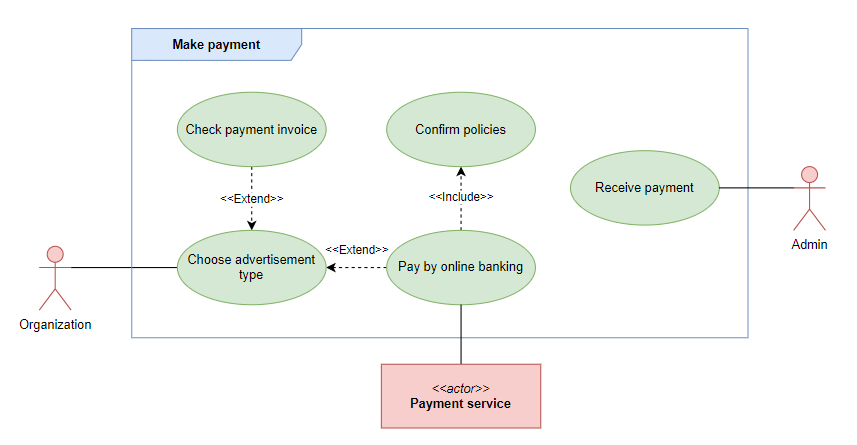
\includegraphics[width=0.7\textwidth]{Figures/payment_ucd.png}
\caption{Use-case diagram of the make payment function}
\label{fig:payment-activity-diagram}
\end{figure}


\begin{longtblr}[
    caption = {Use Case: Make payment},
    label = {tblr:make_payment_use_case},
  ]{
    vline{1-10} = {-}{},
    hline{-} = {1-2}{},
    colspec={X[3,l] X[7, l]},
  }
  \textbf{Use-case name} & \textbf{Make payment} \\
  \textbf{Actors} & {
    Organization, Admin, Payment service
  } \\
  \textbf{Preconditions} & {
    Organizations create a blog successfully.
  } \\
  \textbf{Postconditions} & {
    1. Organizations have blogs that have the correct advertisement duration.
    \\2. Admins receive payment from organizations.
  } \\
  \textbf{Triggers} & {
    Organizations apply advertisements on their blogs.
  } \\
  \textbf{Normal flow} & {
    1. The system shows all advertisement types with their periods.
    \\2. Users choose a type of advertisement. The system shows the payment invoice.
    \\3. Users confirm all the payment policies and finish the payments.
    \\4. Payment service processes the transactions.
    \\5. Admins receive the payments from the organizations.
    \\6. System notifies organizations and admins of successful payments.
  } \\
  \textbf{Alternative flows} & {
    Alternative flow 1, at step 3:
    \\3. Users can refuse the payment policies and stop the payments.
    \\Alternative flow 2, from step 4:
    \\4. Payment service processes the transactions and gets errors.
    \\5. System notifies organizations of failed payments.
  } \\
  \textbf{Exceptions} & {
    1. Organizations do not use the supported payment service.
    \\2. The balances in the accounts of organizations are not enough.
    \\3. Internal errors in the payment service occur.
  } \\
\end{longtblr}


\subsection{Manage blogs}

\begin {figure}[H]
\centering
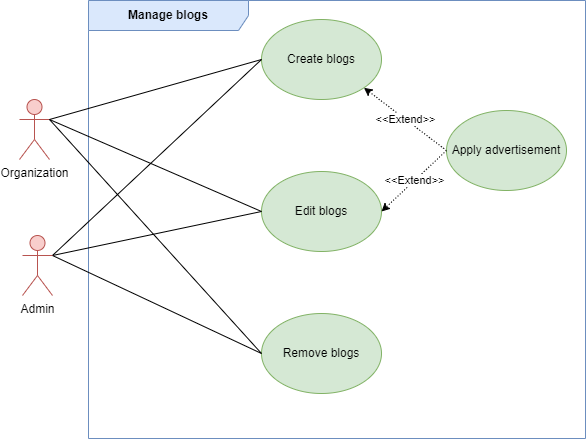
\includegraphics[width=0.7\textwidth]{Figures/manage_blog_ucd.png}
\caption{Use-case diagram of the manage blogs function}
\label{fig:manage-blog-activity-diagram}
\end{figure}

\begin{longtblr}[
    caption = {Use Case: Manage Blogs},
    label = {tblr:manage_blogs},
  ]{
    vline{1-14} = {-}{},
    hline{-} = {1-2}{},
    colspec={X[3,l] X[7, l]},
  }
  \textbf{Use-case name}     & \textbf{Manage blogs}                                           \\
  \textbf{Actors}            & Organization, Admin                                             \\
  \textbf{Preconditions}     & Organizations logged successfully into the system.              \\
  \textbf{Postconditions}    & Organizations can create and edit their blogs.                  \\
  \textbf{Triggers}          & Organizations access the blog management section of the system. \\
  \textbf{Normal flow}       & {
      1. Organizations click on the add blogs button of the system. The system displays a blog form screen.
  \\2. Organizations provide and submit blog creation forms.
  \\3. The system creates new blogs.
  }                                                                                            \\
  \textbf{Alternative flows} & {
      Alternative flow 1: from step 1:
  \\1. Organizations choose to update blogs. The system displays a blog form screen.
  \\2. Organizations provide and submit blog update forms.
  \\3. The system updates the blogs.
  \\Alternative flow 2 (for both normal flow and flow 1), from step 3:
  \\4. Organizations apply advertisement on blogs.
  \\5. The system updates the blogs to advertisement blogs.
  }                                                                                            \\
  \textbf{Exceptions}        &                                                                 \\
\end{longtblr}


\section{Workflow analysis}
\subsection{Activity Diagrams}

\subsubsection{Self Registration}

The use case starts when a user accesses the register page (or clicks the register button on the login form), and then a register form will be displayed. The user provided some information (including email, password, and name). Then,  the provided information is verified. If it is valid, a confirmation email will be sent to the user. After accessing the link in the email, a new account is created and the user can log into the system.

\begin{figure}[H]
  \centering
  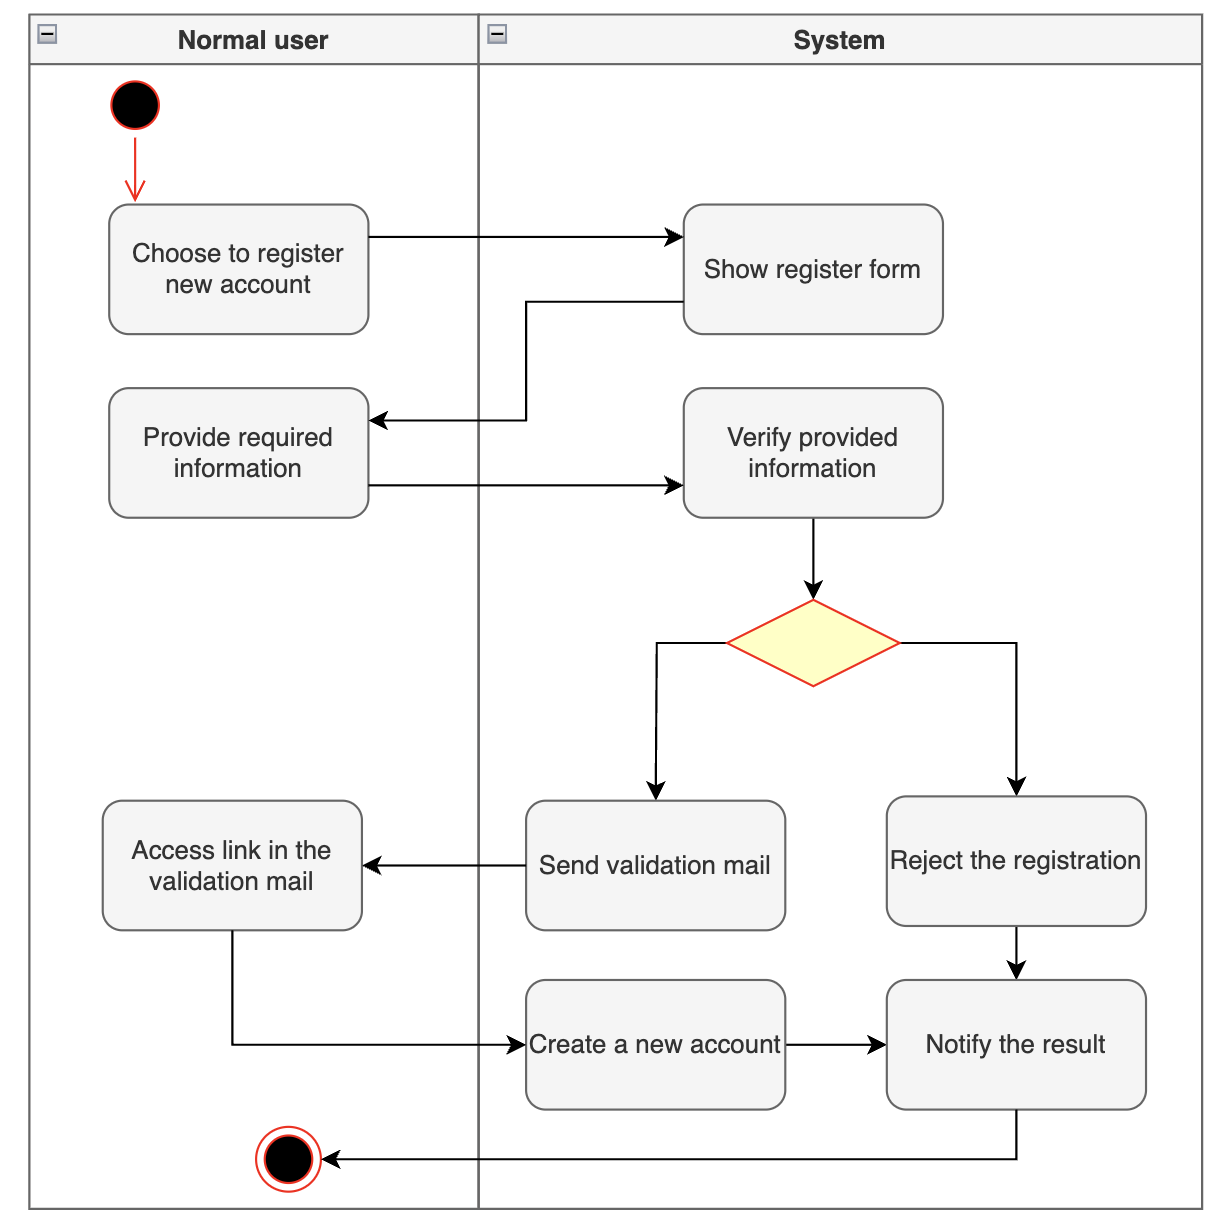
\includegraphics[width=0.7\textwidth]{Figures/self_register.png}
  \caption{Self Registration activity diagram}
  \label{fig:self-registration}
\end{figure}


\subsubsection{Login}

The use case starts when an unauthorized user tries to access internal features or goes to the login page. The user at the login can provide an email and password and send them to the system. If the credential information is valid, the user will be granted access permission and navigated to an internal page. Otherwise, an error alert will be displayed.

\begin{figure}[H]
  \centering
  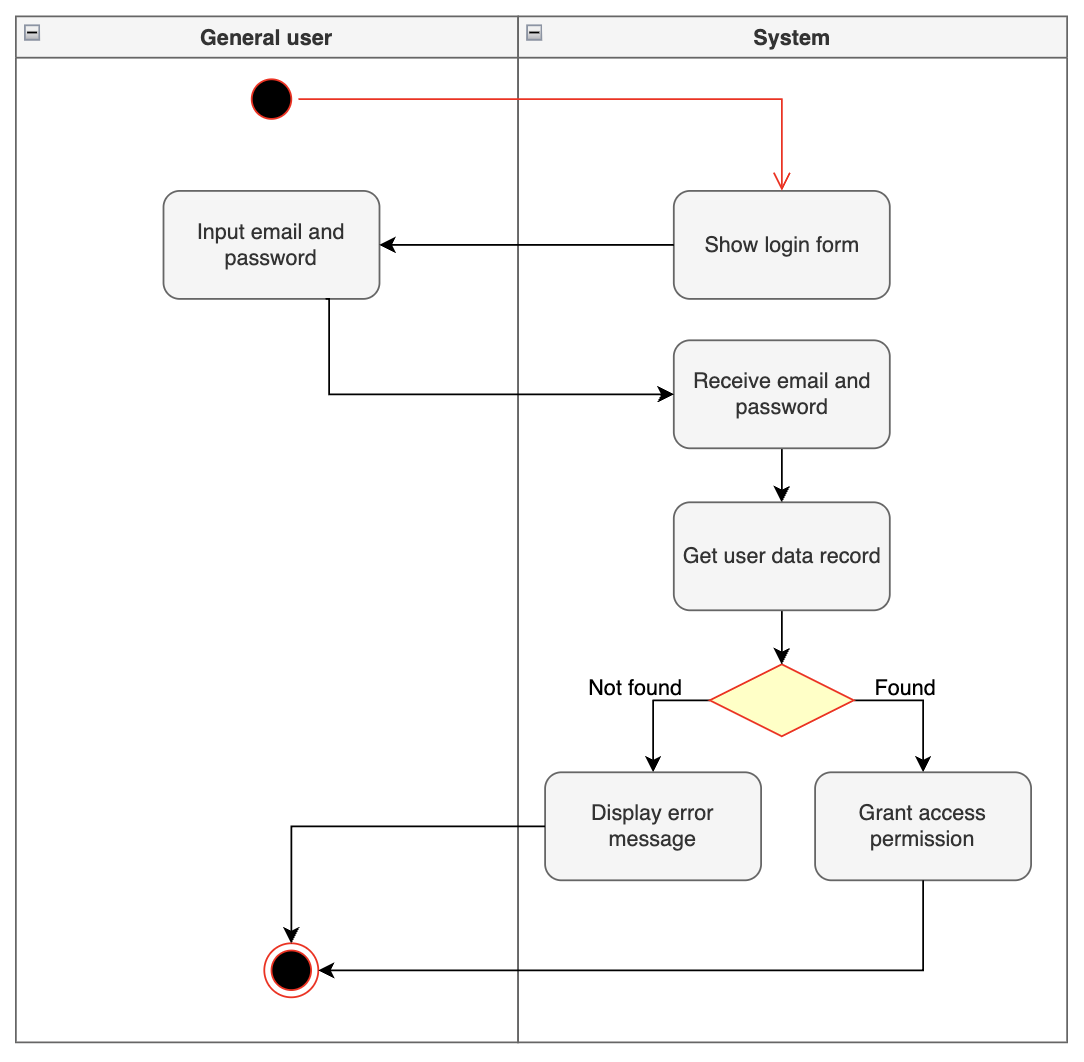
\includegraphics[width=0.7\textwidth]{Figures/login.png}
  \caption{Login activity diagram}
  \label{fig:login}
\end{figure}

\subsubsection{Login with a Google account}

The use case starts when a user chooses the option of logging in with a Google account, then a Google login form will be displayed. Users provide Google authentication information. Google Auth service verifies the authentication information and generates an access token. Finally, the system validates the access token and grants access permission to the user.

\begin{figure}[H]
  \centering
  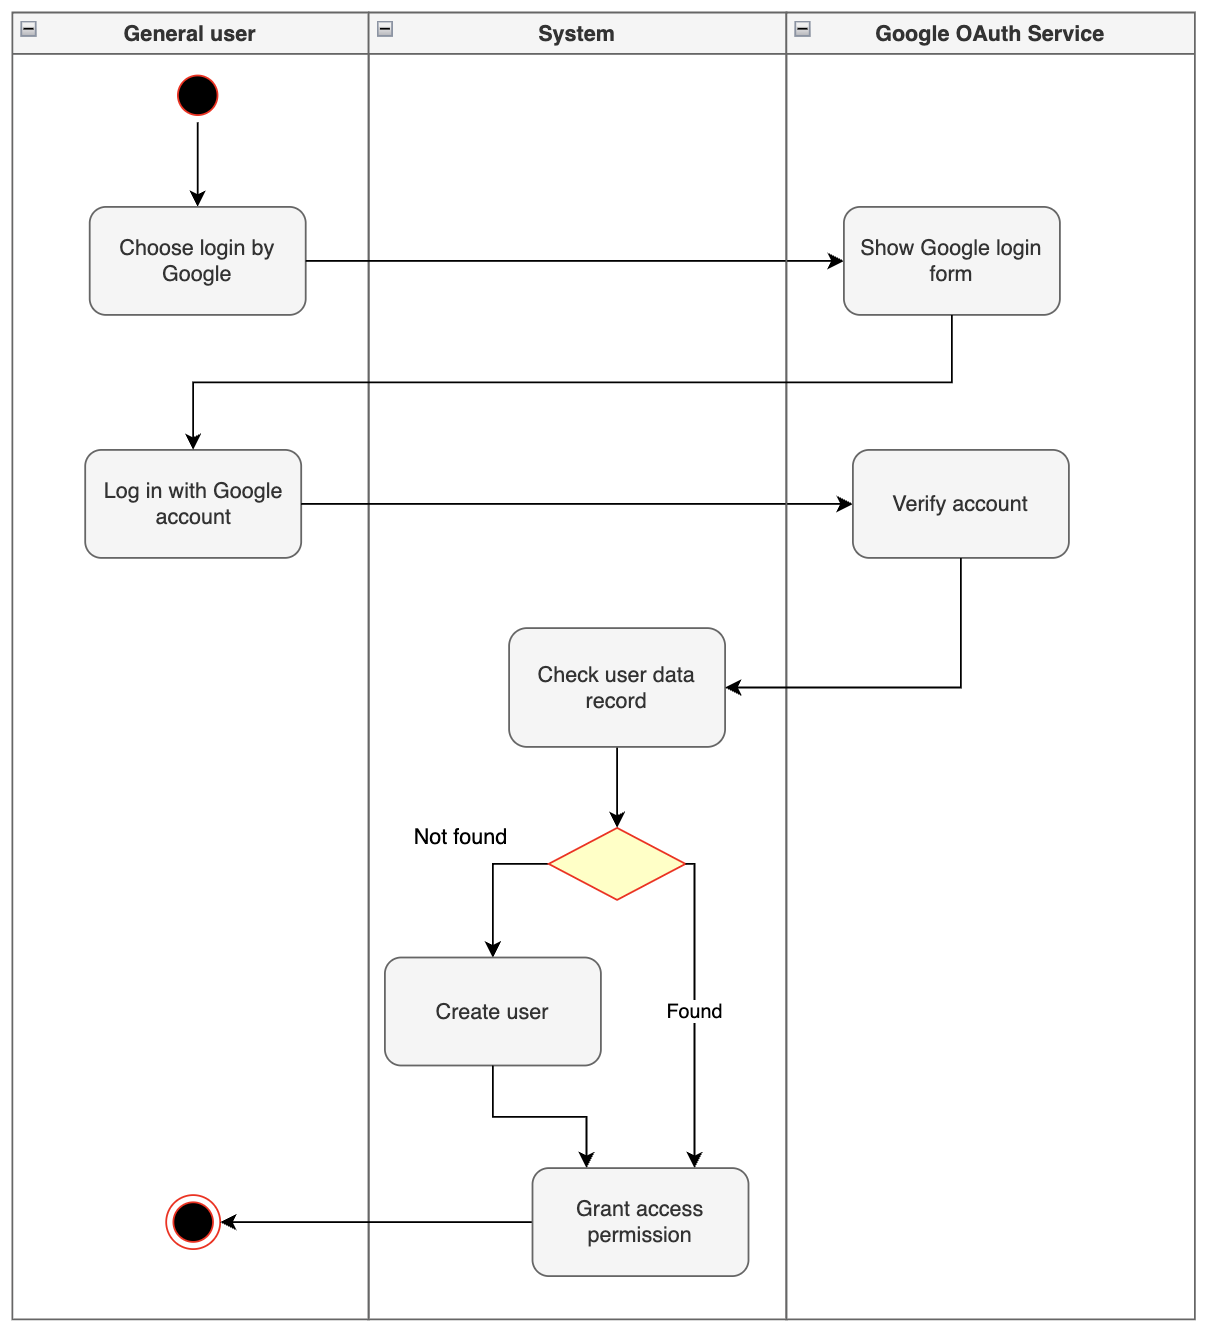
\includegraphics[width=0.7\textwidth]{Figures/login_gg.png}
  \caption{Login with a Google account activity diagram}
  \label{fig:login-google}
\end{figure}

\subsubsection{Update to Organization account}

The use case starts when an individual user chooses to update to organization accounts, then a form will be displayed. Then, users provide some information for verification and submit them. After the update-account application is verified by admins, the system updates the account and notifies the user of the results.

\begin{figure}[H]
  \centering
  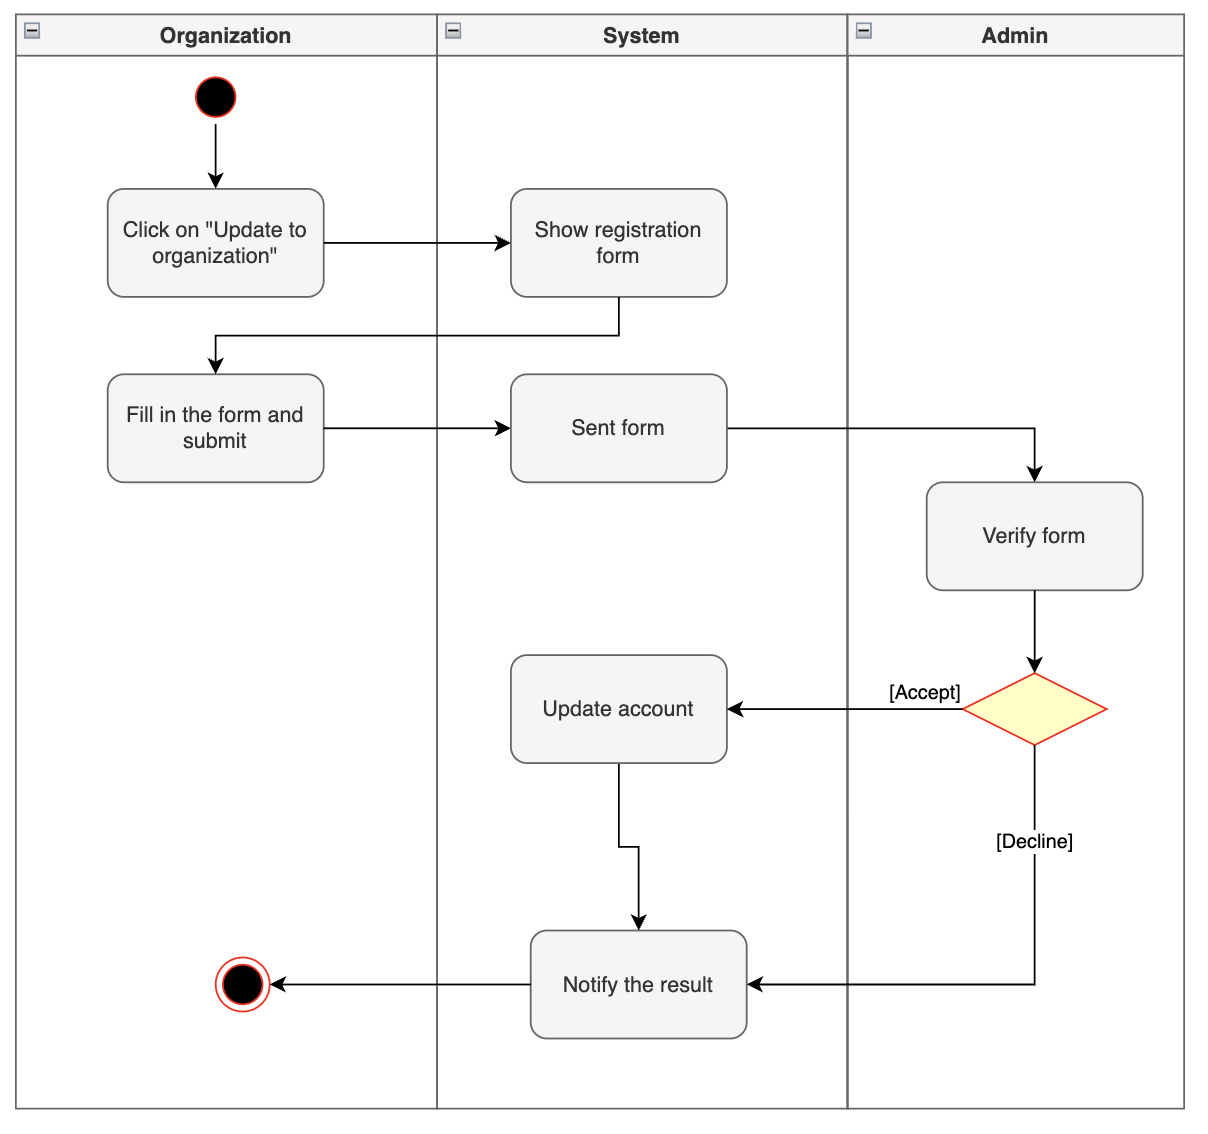
\includegraphics[width=0.7\textwidth]{Figures/update_org.png}
  \caption{Update to Organization account activity diagram}
  \label{fig:update-org}
\end{figure}

\subsubsection{Manage pet profile}

The use case starts when a user accesses the pet profile management page. The user chooses to edit or create a new profile and a form will be displayed. Note that the form would be filled if the user chose to edit an available profile. In that case, the user can modify the fields or rather delete the profile. Otherwise, the user can input the pet information and submit it. The user can also fill in pet breeds and colors by providing images. Finally, the content of the form will be verified, and the result will be displayed.

\begin{figure}[H]
  \centering
  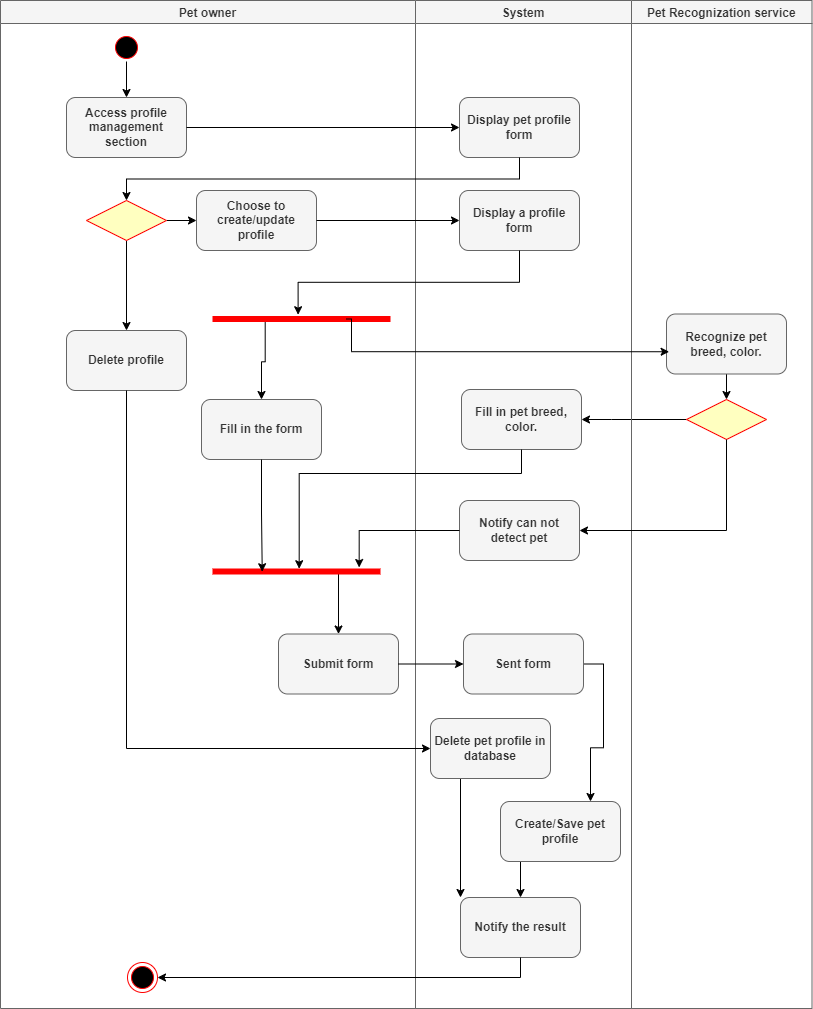
\includegraphics[width=0.7\textwidth]{Figures/manage_pet.png}
  \caption{Manage pet profile activity diagram}
  \label{fig:manage-pet}
\end{figure}

\subsubsection{Access pet profile}

In the pet profile page, a user has options to find pets by filtering by categories or providing pet images. In case the user filters by images, those images will be processed by the Pet Recognition Service. Then, the filtered pet profiles will be displayed to the user. The user can click on pet profiles for further information or continue finding other pet profiles.

\begin{figure}[H]
  \centering
  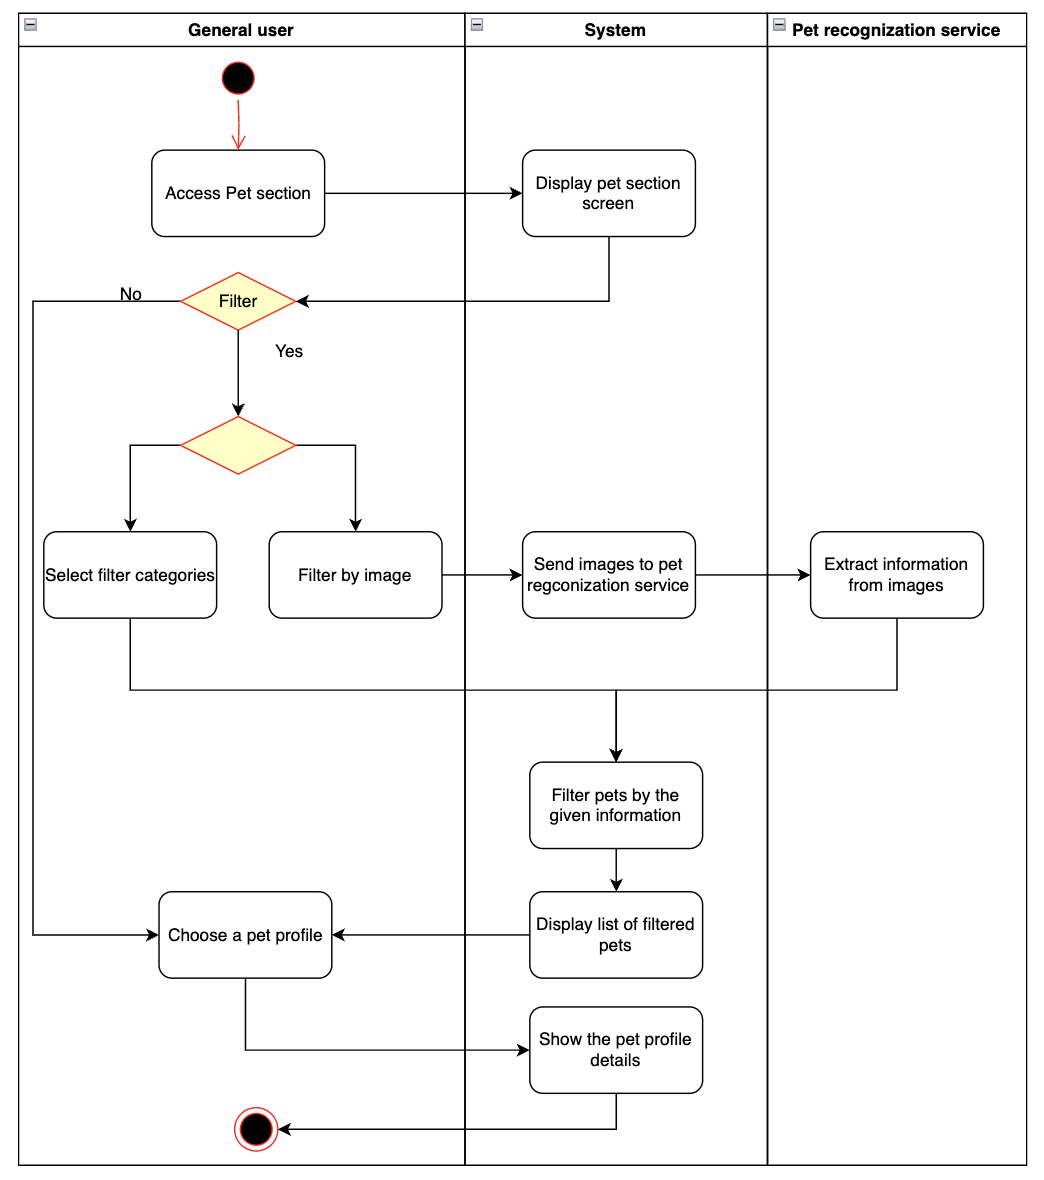
\includegraphics[width=0.7\textwidth]{Figures/access_pet.png}
  \caption{Access pet profile activity diagram}
  \label{fig:access-pet}
\end{figure}

\subsubsection{Adopt pets}

After finding a pet profile successfully, if the pet is still available, a user can choose to adopt the pet by filling in the required information in the adoption form and sending it. The application form will be reviewed by the pet owner. The result will be sent to the user then. Note that, the user can still contact directly to the pet owner during the pet adoption process.

\begin{figure}[H]
  \centering
  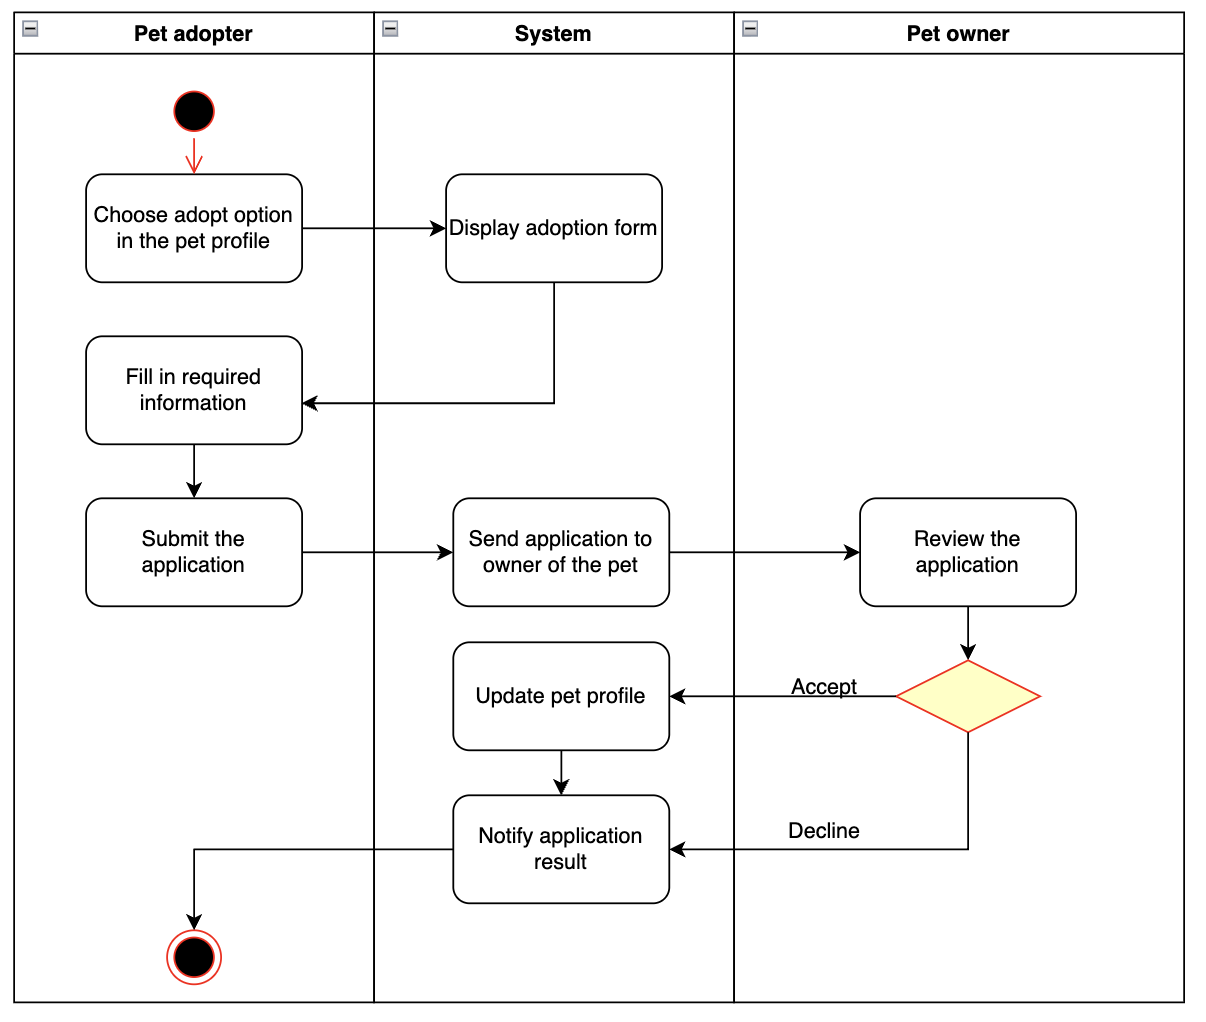
\includegraphics[width=0.7\textwidth]{Figures/adopt_pet.png}
  \caption{Adopt pets activity diagram}
  \label{fig:adopt-pet}
\end{figure}

\subsubsection{Interact with posts}

After accessing a pet profile successfully, a user can also see public posts of the pet. The user can choose a post for further information and leave their comments or likes on the post. Note that the private posts can only be seen by the pet owner and admins.

\begin{figure}[H]
  \centering
  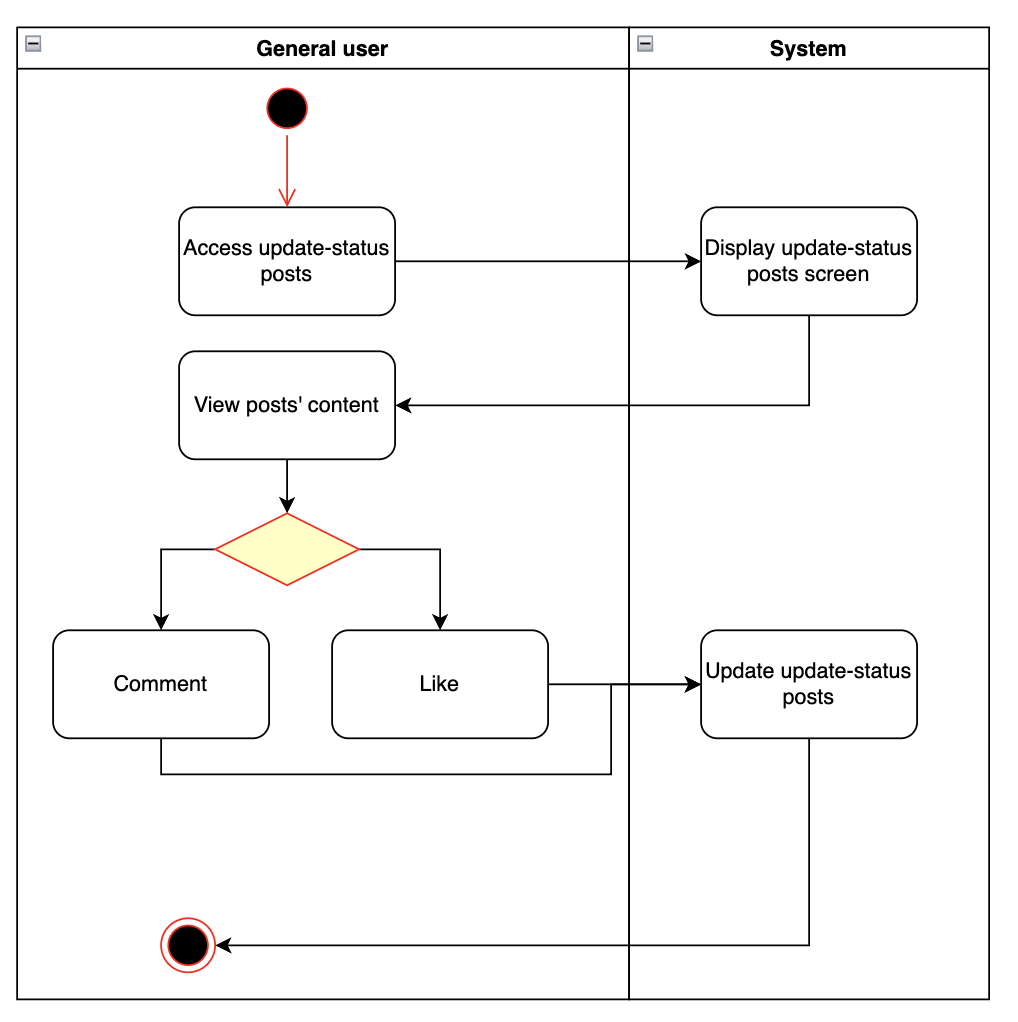
\includegraphics[width=0.7\textwidth]{Figures/post_interact.png}
  \caption{Interact with posts activity diagram}
  \label{fig:interact-post}
\end{figure}


\subsubsection{Update pet status}

Updating the status of a pet is uploading posts about it. The use case starts when an owner can select a pet profile and choose the option of updating the pet status. After filling information, the owner can set visibility for the post. Finally, the user can send the form and a new post is created.

\begin{figure}[H]
  \centering
  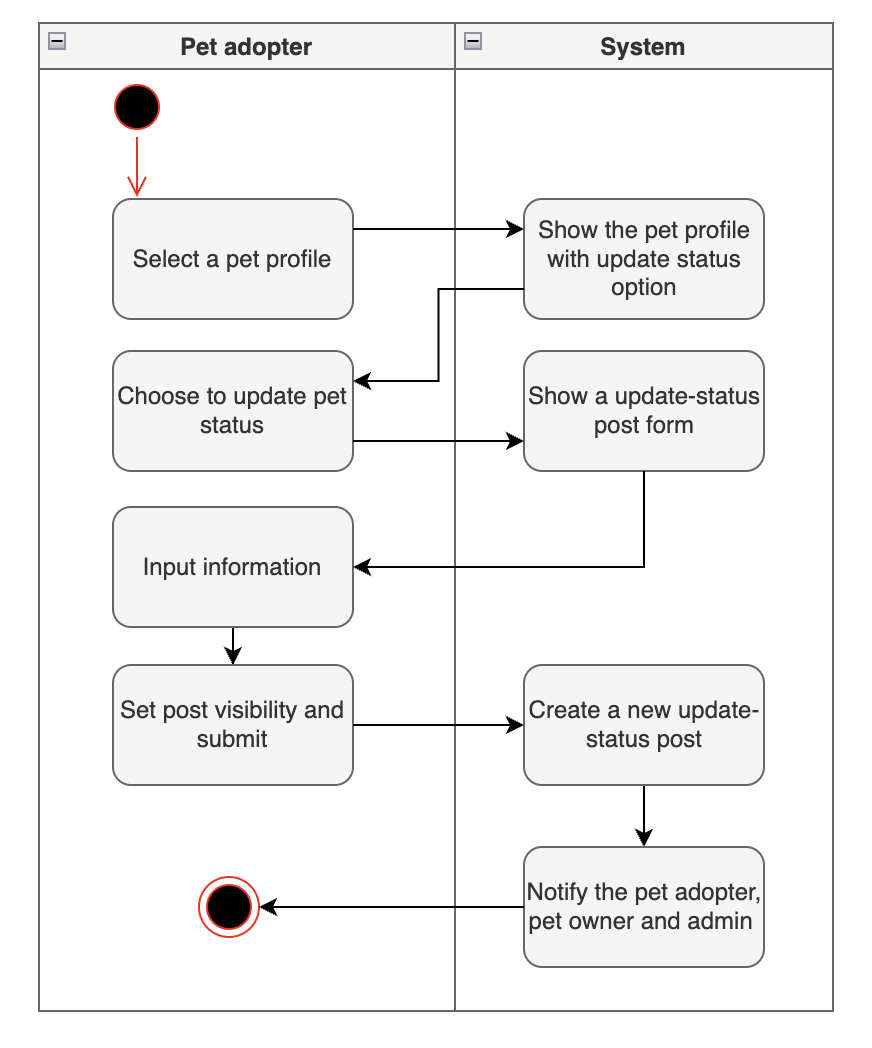
\includegraphics[width=0.7\textwidth]{Figures/pet_status.png}
  \caption{Update pet status activity diagram}
  \label{fig:update-pet-status}
\end{figure}

\subsubsection{Manage blogs for Organizations}

The use case starts when a user with an Organization account accesses the blog management page. The user chooses to edit or create a new blog, then a form will be displayed. Note that the form would be filled if the user chose to edit an available blog. In that case, the user can modify the fields or rather delete the blog. If the user wants to create a new blog, the user can input and submit it. Finally, admins will verify the blog and the result will be sent to the user.

\begin {figure}[H]
\centering
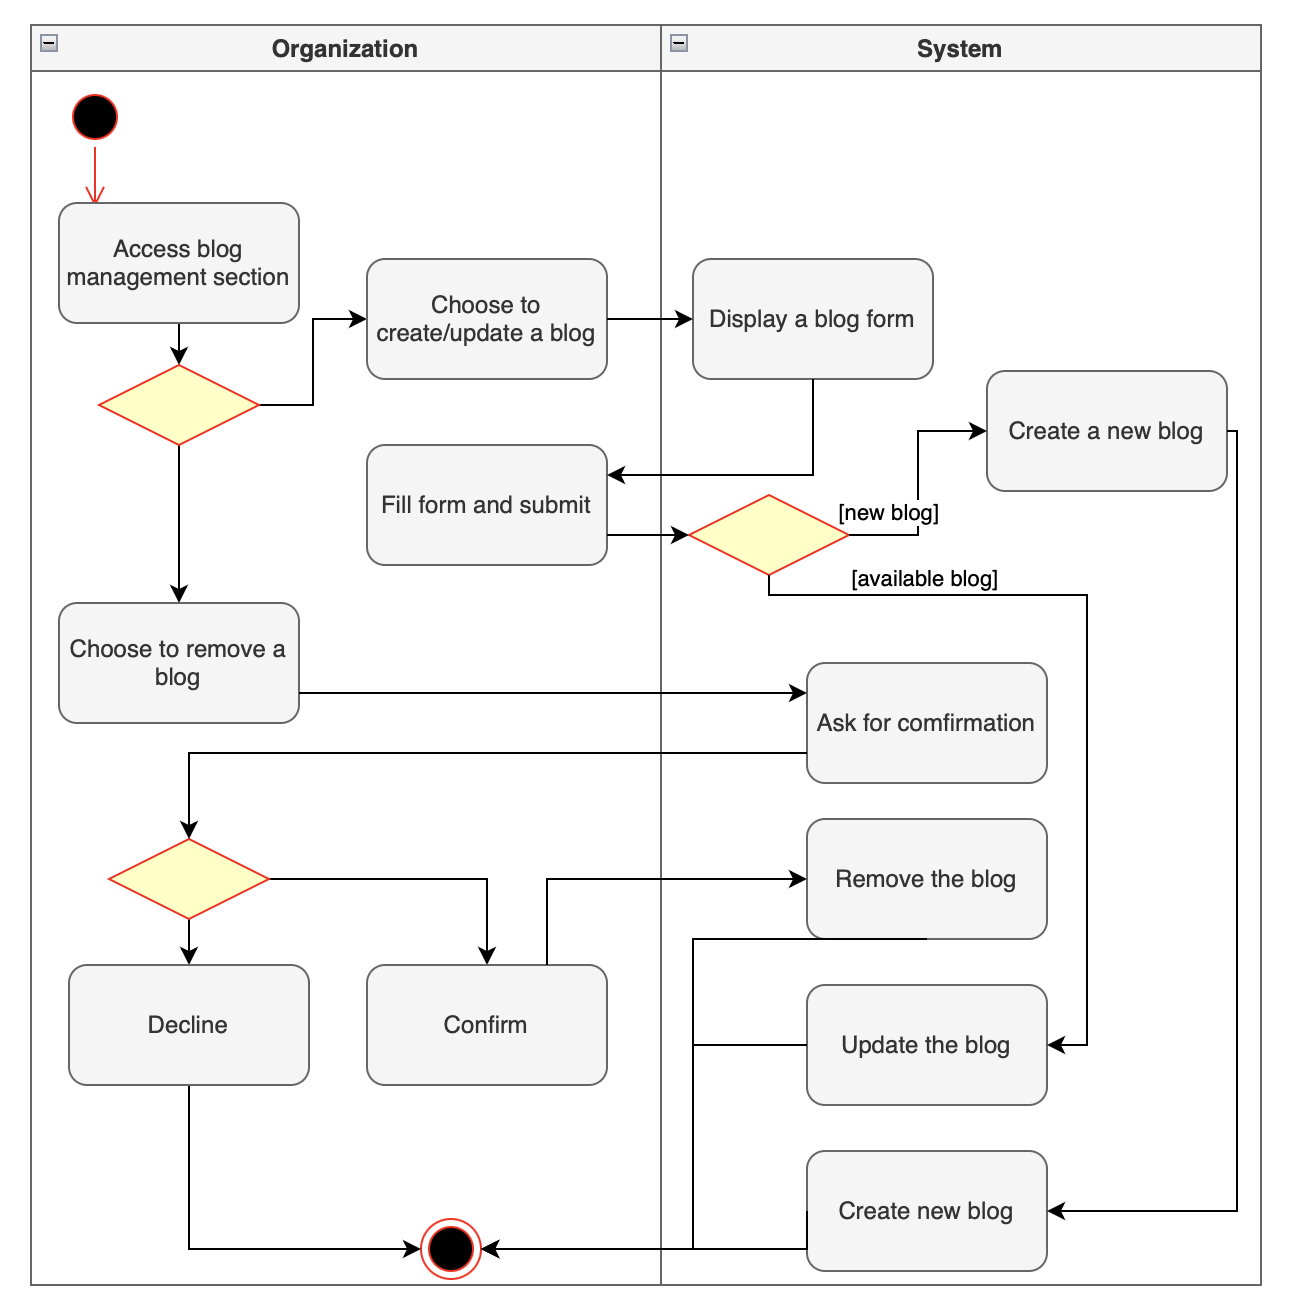
\includegraphics[width=0.7\textwidth]{Figures/manage_blog_org.png}
\caption{Manage blogs for Organizations activity diagram}
\label{fig:manage-blog}
\end{figure}

\subsubsection{Manage blogs for Administrator}

The use case starts when a user with an Organization account accesses the blog management page. The flow is almost the same as for Organization users except that the blog is created without any verification.

\begin {figure}[H]
\centering
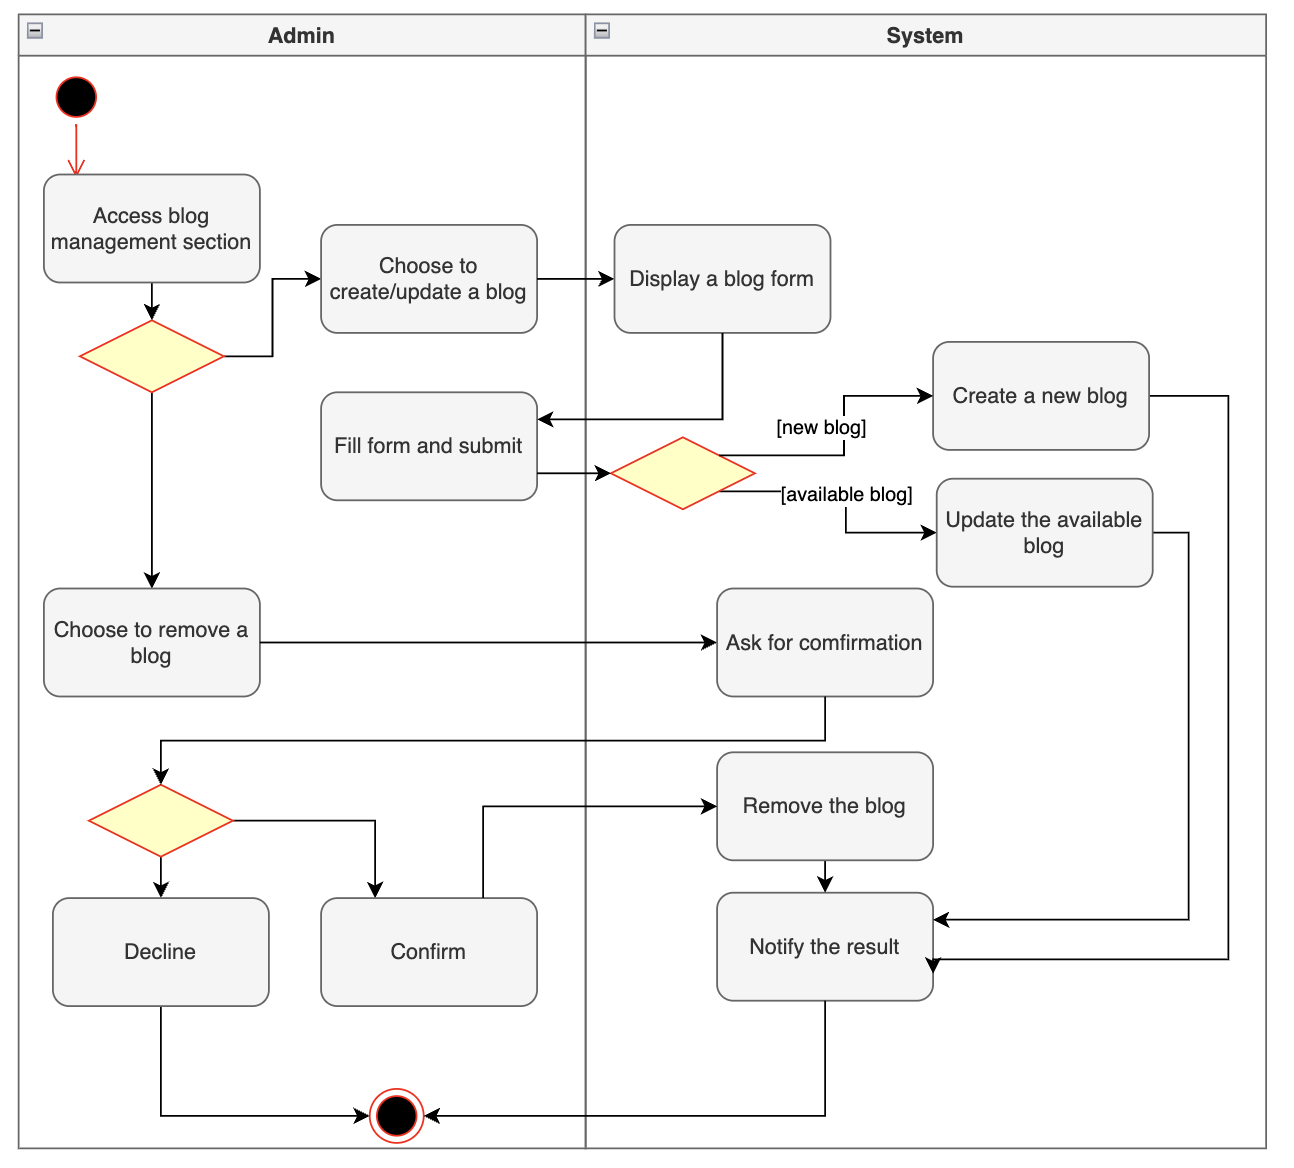
\includegraphics[width=0.7\textwidth]{Figures/manage_blog_admin.png}
\caption{Manage blogs for Administrator activity diagram}
\label{fig:manage-blog-admin}
\end{figure}

\subsubsection{Make payment}

When a user applies an advertisement on a log, the system shows all advertisement types with their periods. Then, users choose a type of advertisement and the system shows the payment invoice. If the user confirms the payment, the Payment service will process the transaction and the result will be displayed to admins and the user.

\begin {figure}[H]
\centering
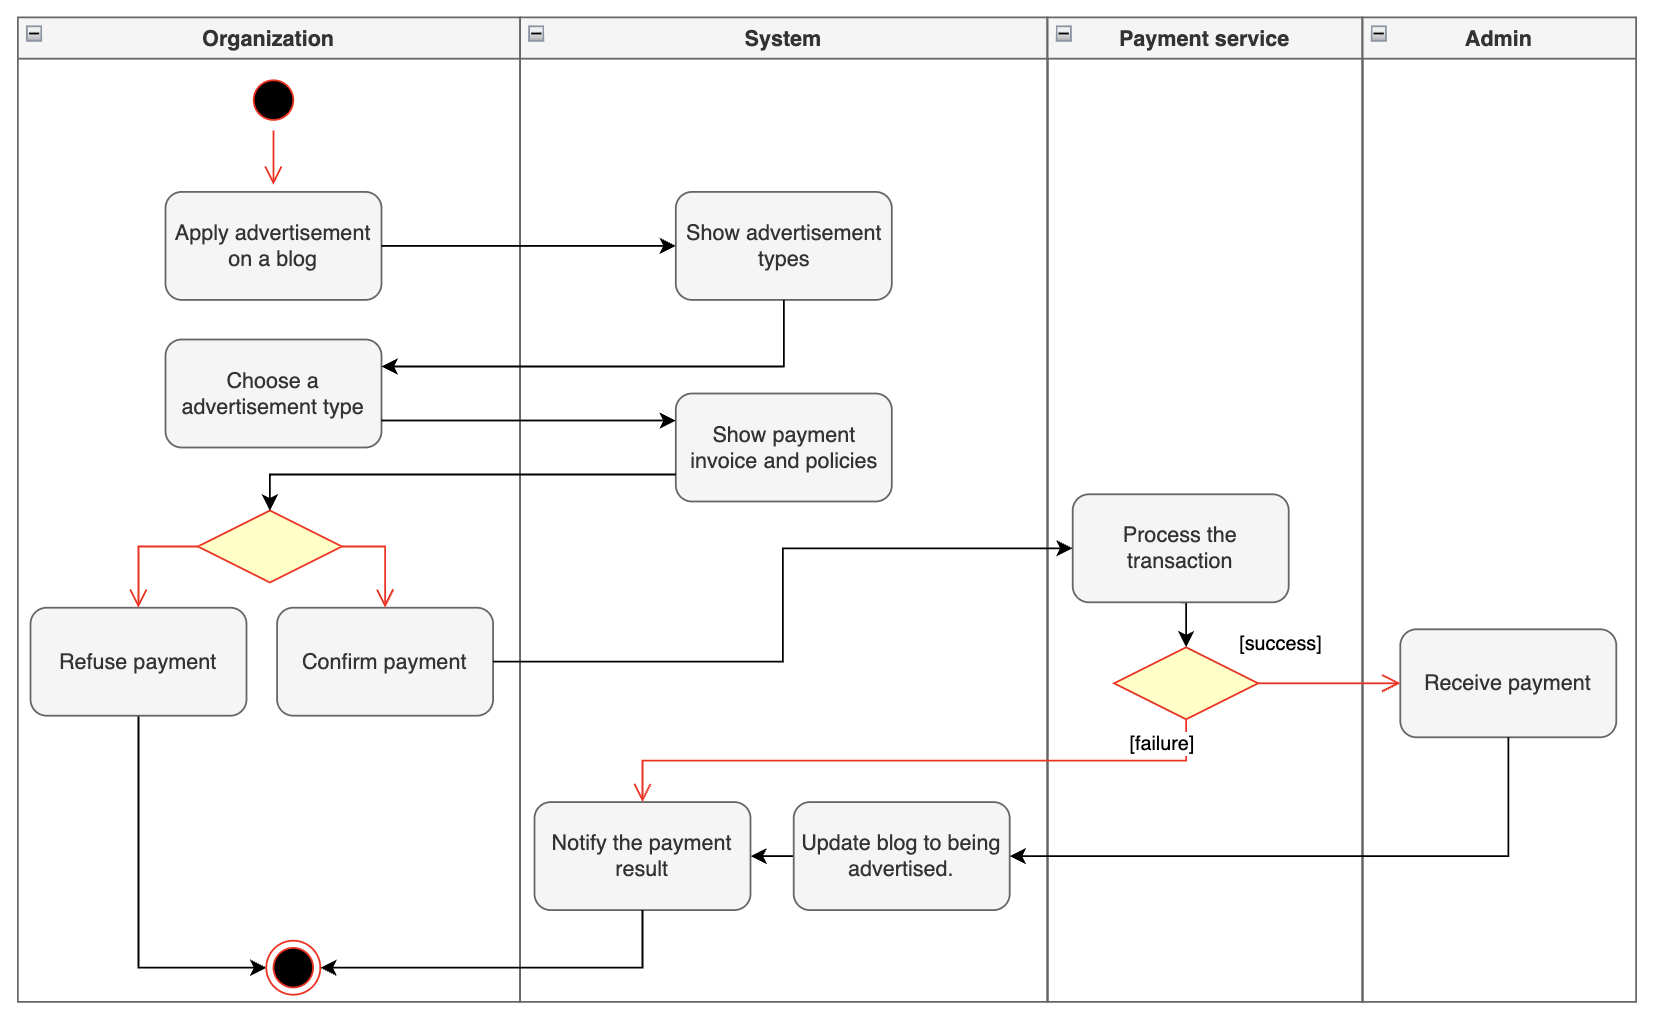
\includegraphics[width=0.7\textwidth]{Figures/payment.png}
\caption{Make payment activity diagram}
\label{fig:make-payment}
\end{figure}

\subsection{Class Diagrams}

The system design is expected to adhere to the Layered and Repository
design patterns as outlined in \emph{\textbf{section 3.1}}.
Consequently, the system's classes are categorized into four distinct
groups.

\emph{View Classes} (Figure 21): These classes encompass the user
interface and user experience (UI/UX) components, along with methods for
handling user events. Each class inherits from a common class,
\emph{BaseLayout}, which encapsulates the components and methods shared
across all view classes.

\emph{Service Classes} (Figure 22): These classes contain methods for
processing the system's logic and business flow. Each class has a
specific responsibility and inherits from a class called
\emph{BaseService}, which encapsulates the methods and services common
to all service classes. The methods of service classes are made
available to view classes via an Application Programming Interface
(API).

\emph{DataLayer Classes} (Figure 23): Each class corresponds to a system
entity in the database. All DataLayer classes inherit from a class
called \emph{BaseDataLayer}, which provides all the methods needed to
interact with the database. It's important to note that a DataLayer
class can only interact with its corresponding entity in the database.

\emph{UnitOfWork} Class (Figure 23): This singular class contains
properties that are instances of DataLayer classes. The BaseService
class implements the UnitOfWork, enabling all service classes to access
the database. This class also includes methods to save changes or
rollback transactions in case of any exceptions at the end of an
application process.

This structure ensures a clear separation of concerns, promoting
maintainability and scalability in the system design.

\begin{figure}[H]
  \centering
  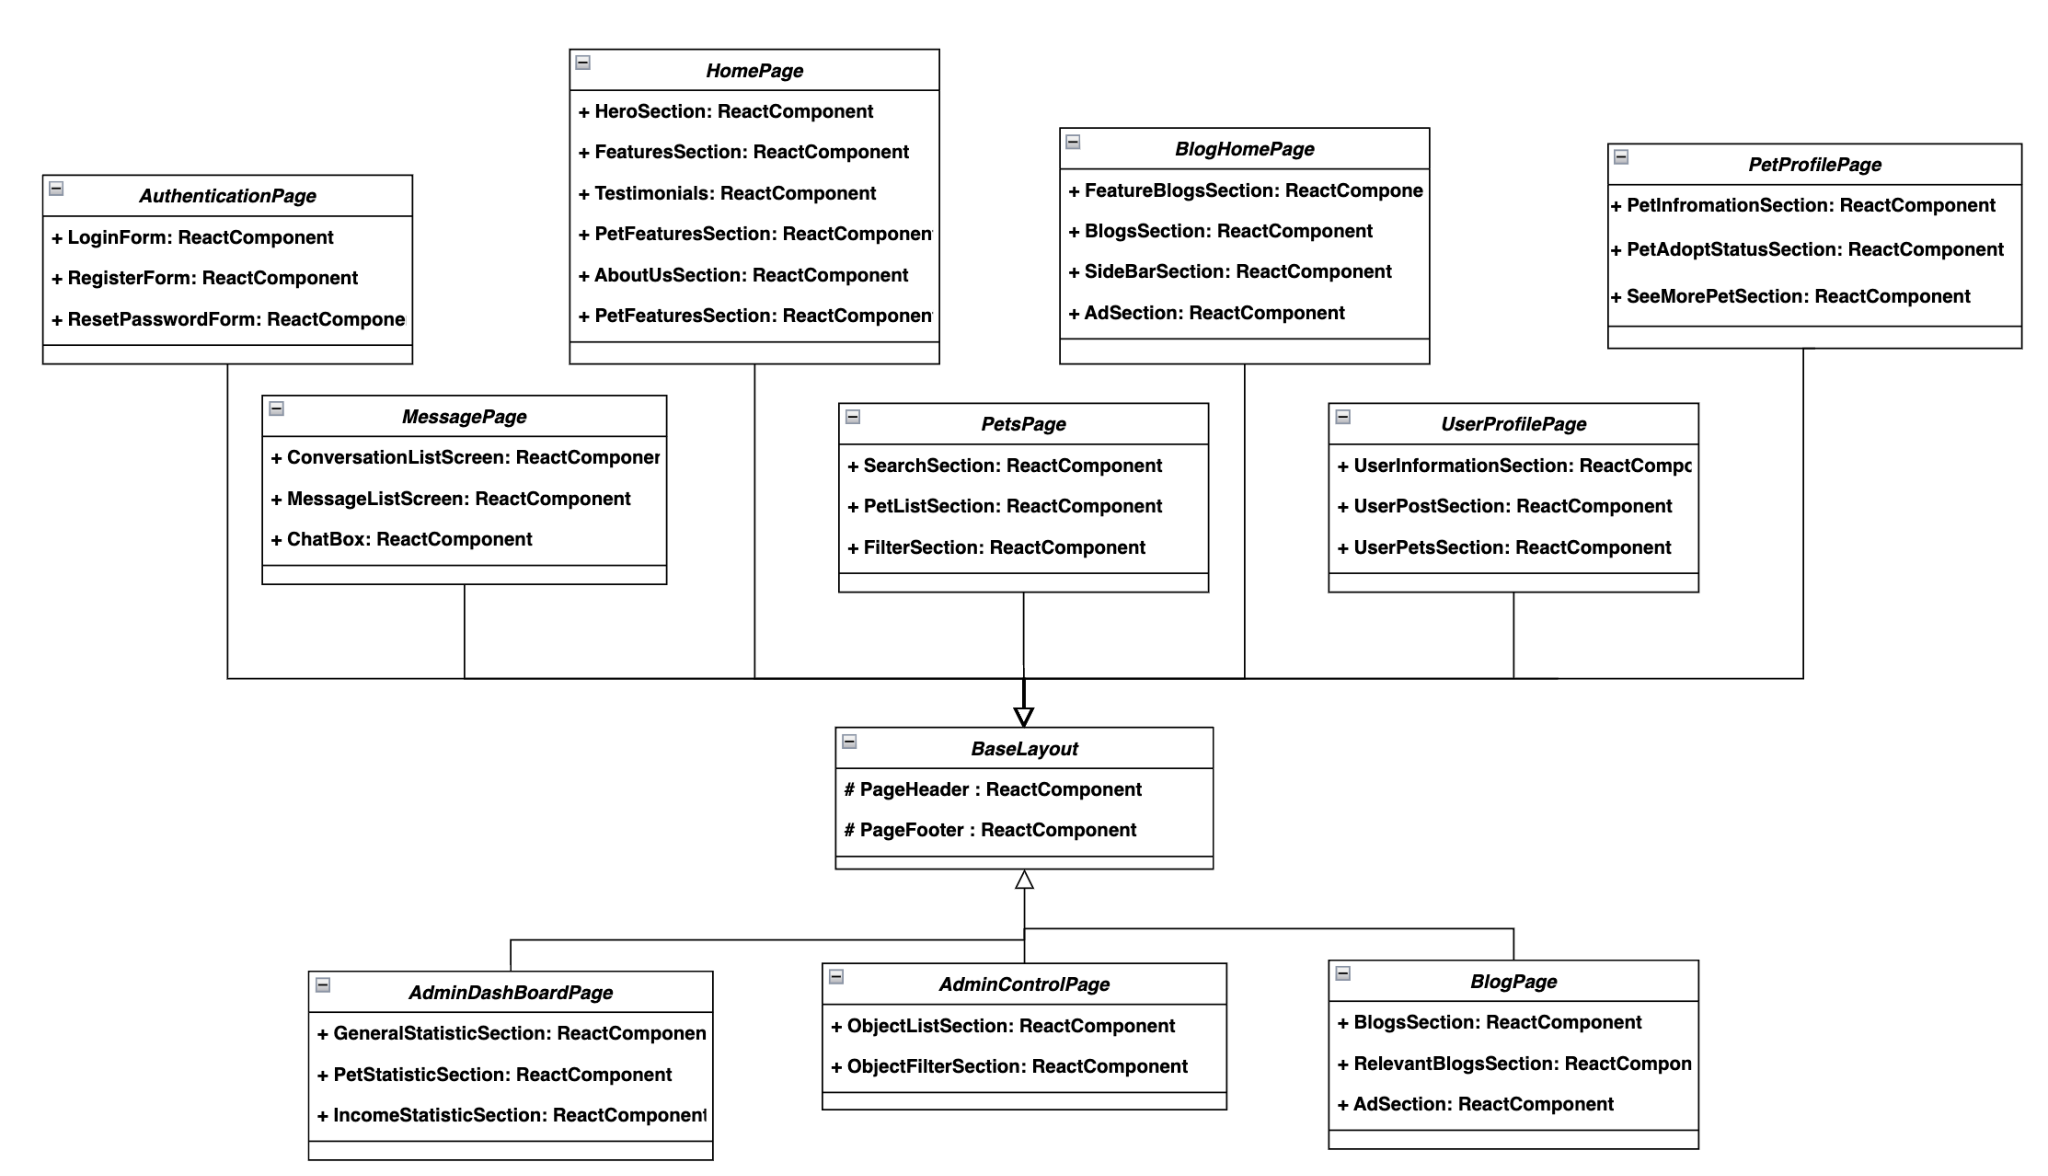
\includegraphics[angle=-90,width=0.8\textwidth]{Figures/view_class.png}
  \caption{View Classes}
  \label{fig:view-classes}
\end{figure}
\clearpage

\begin{figure}[H]
  \centering
  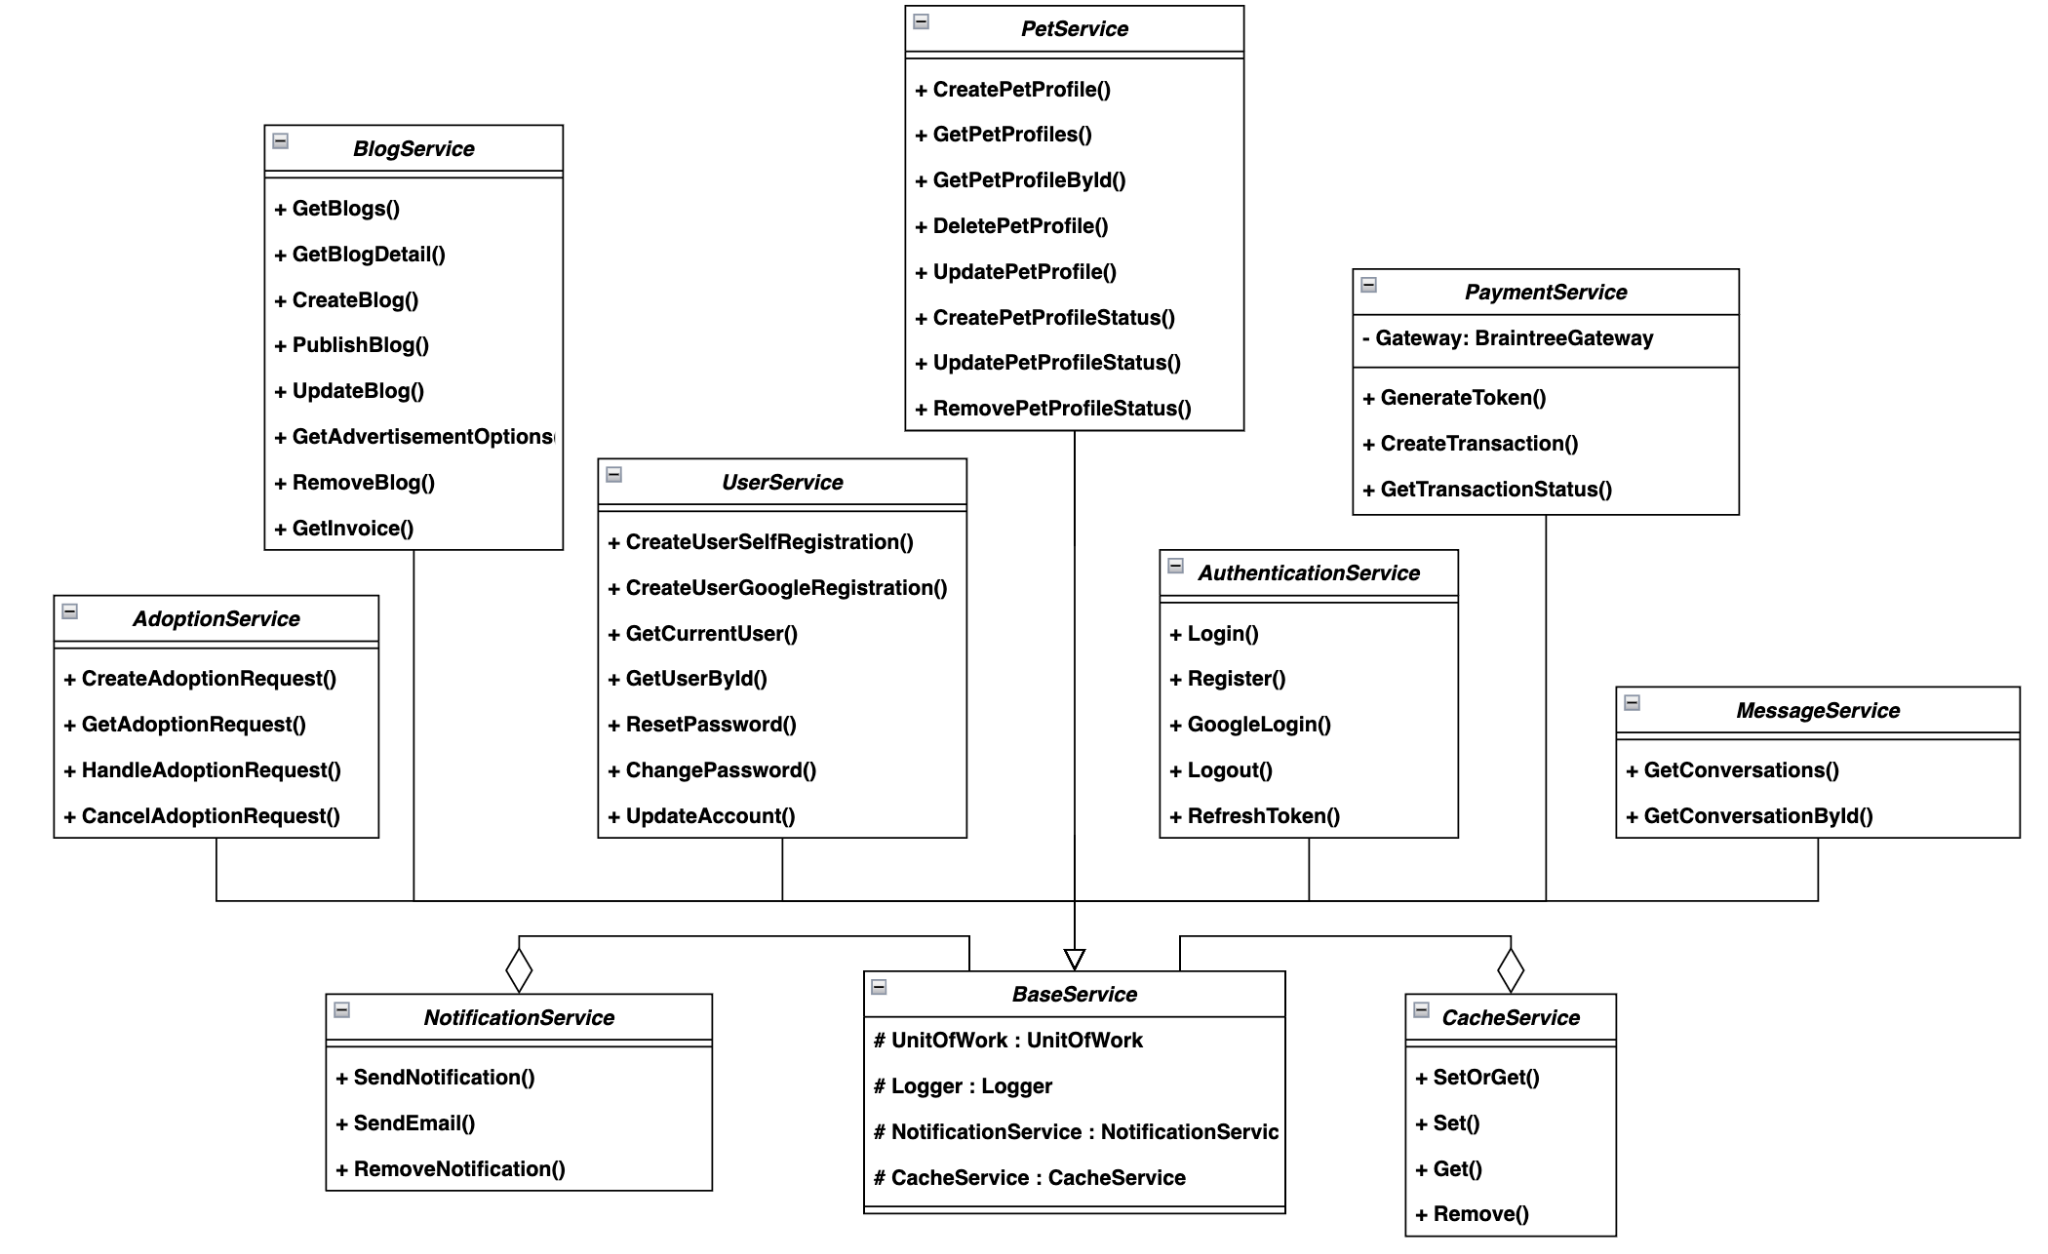
\includegraphics[angle=-90,width=0.8\textwidth]{Figures/service_class.png}
  \caption{Service Classes}
  \label{fig:service-classes}
\end{figure}

\begin{figure}[H]
  \centering
  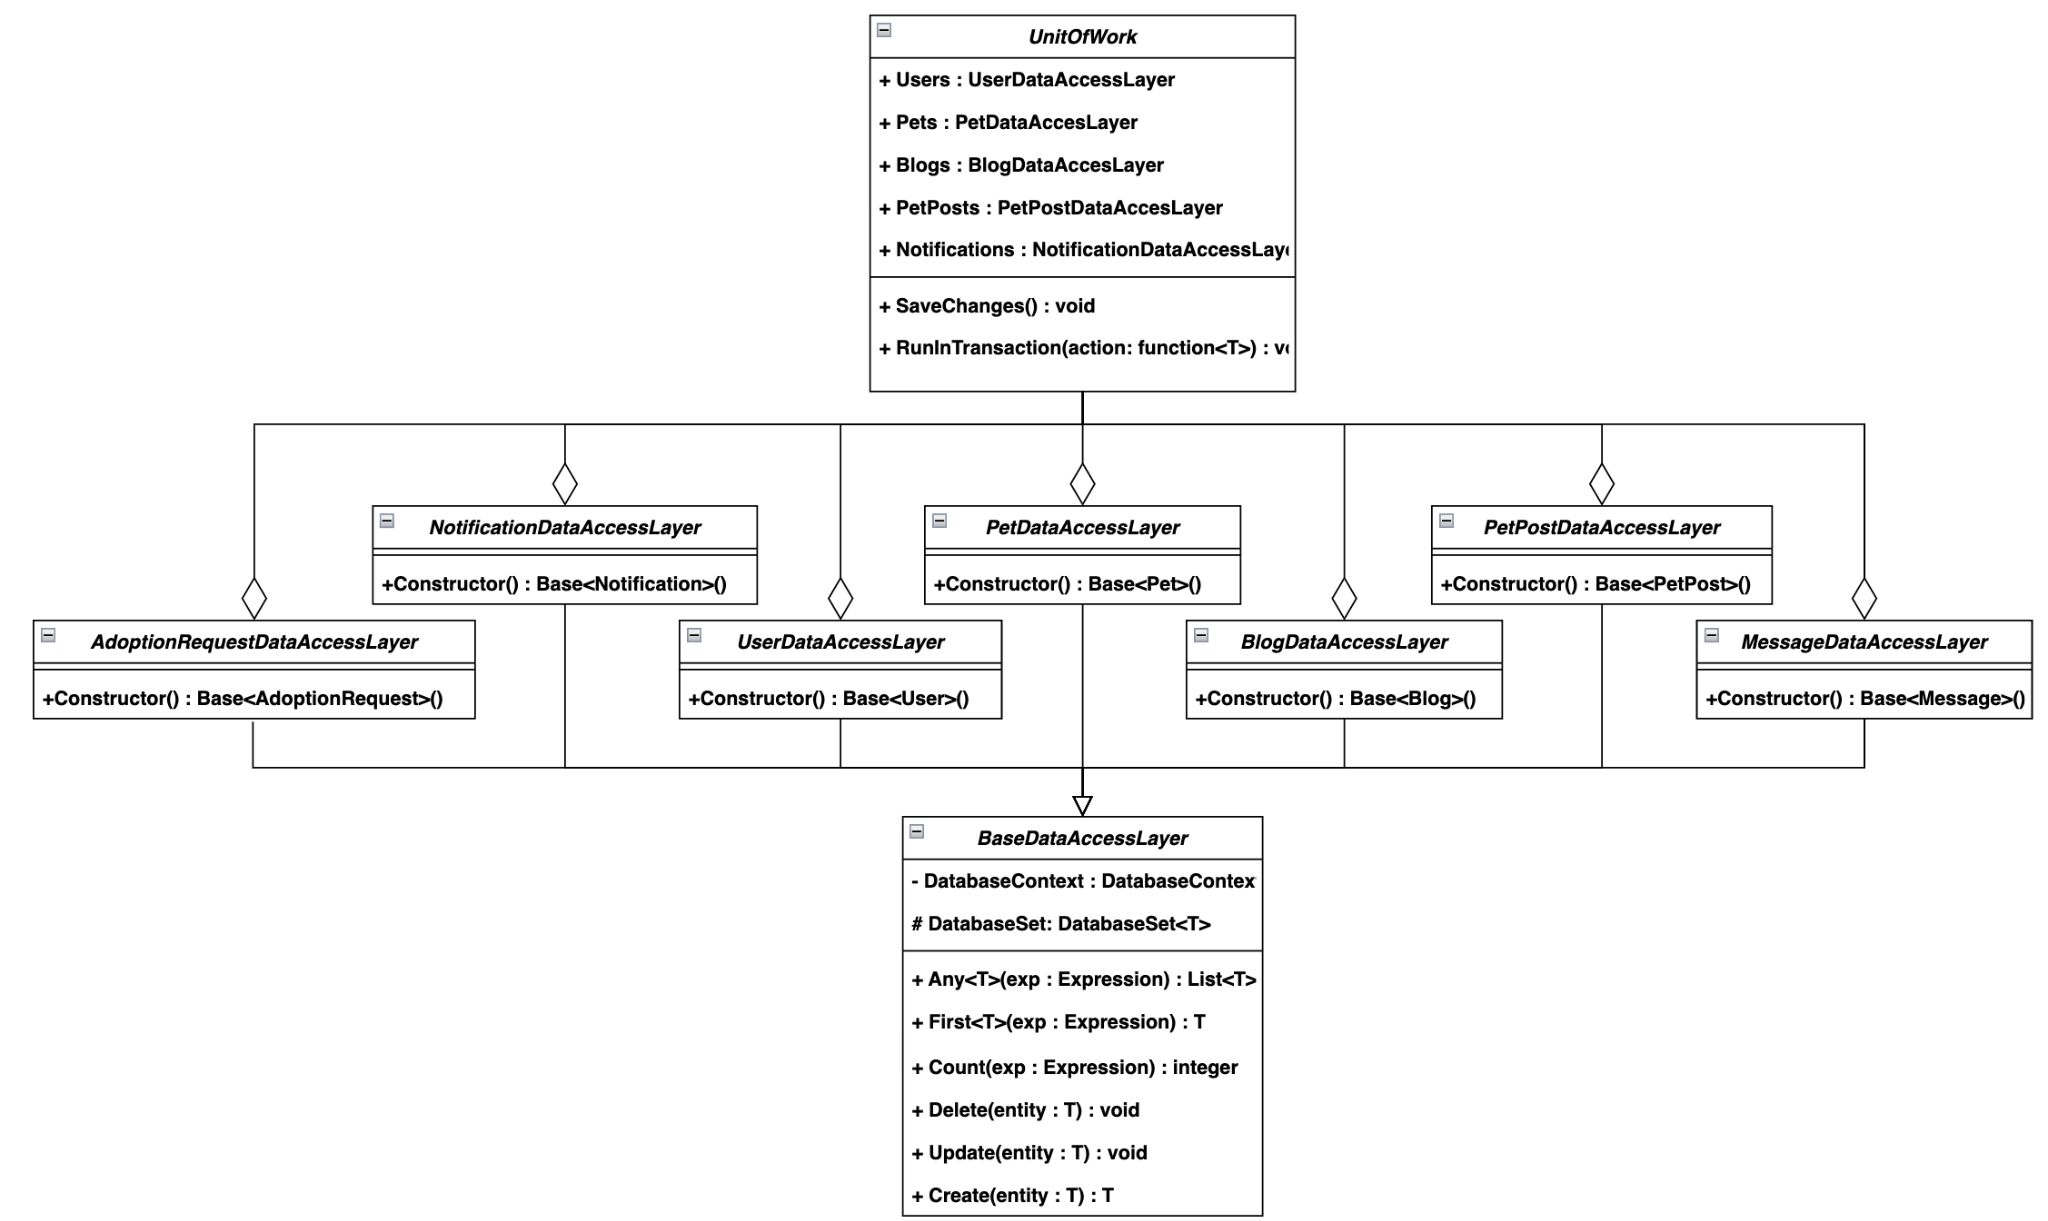
\includegraphics[angle=-90,width=0.8\textwidth]{Figures/uow_class.png}
  \caption{DataLayer Classes}
  \label{fig:datalayer-classes}
\end{figure}
\clearpage

\subsection{Sequence Diagrams}

After completing the class diagrams and activity diagrams of the system, we will  demonstrate how the system's classes interact with each other according to the system's business flow using sequence diagrams.

\subsubsection{Self Registration}

\begin{figure}[H]
  \centering
  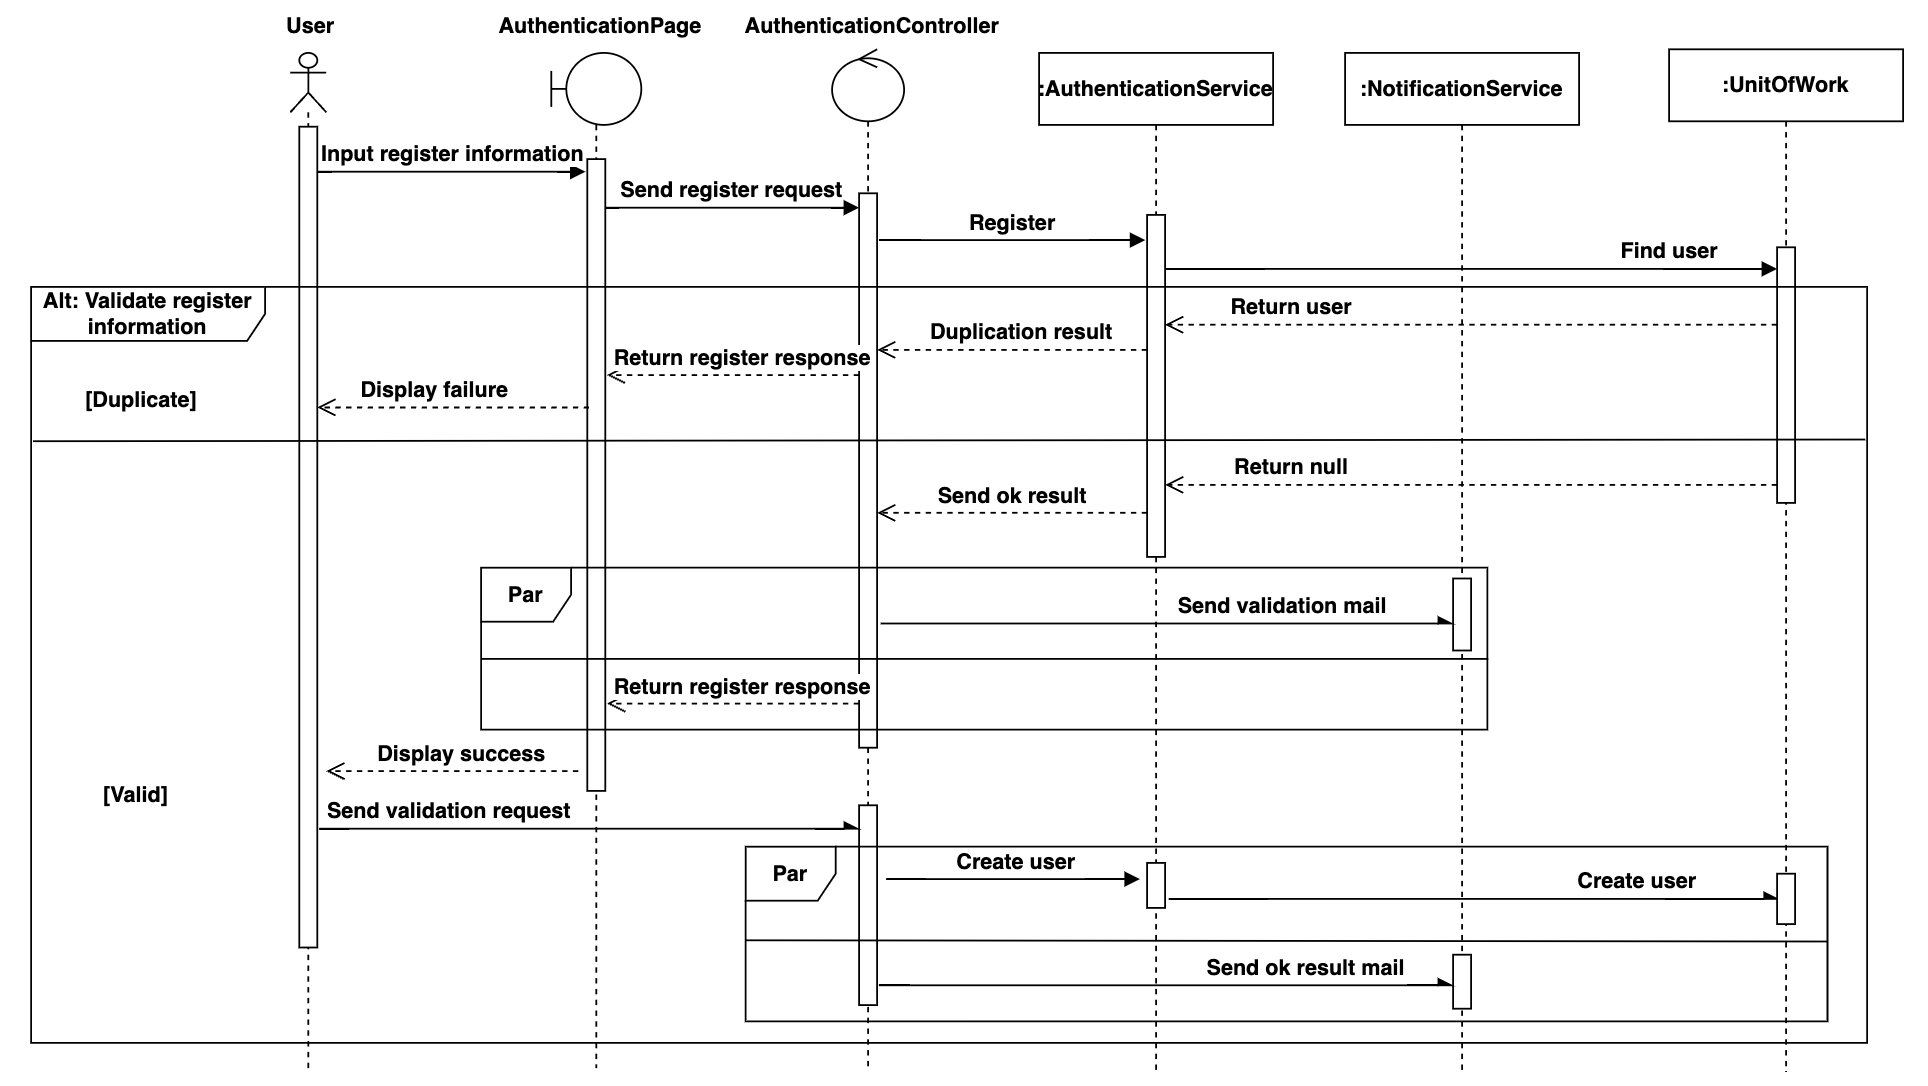
\includegraphics[width=0.9\textwidth]{Figures/self_register_seq.png}
  \caption{Self Registration sequence diagram}
  \label{fig:self-registration-seq}
\end{figure}


\subsubsection{Login}

\begin{figure}[H]
  \centering
  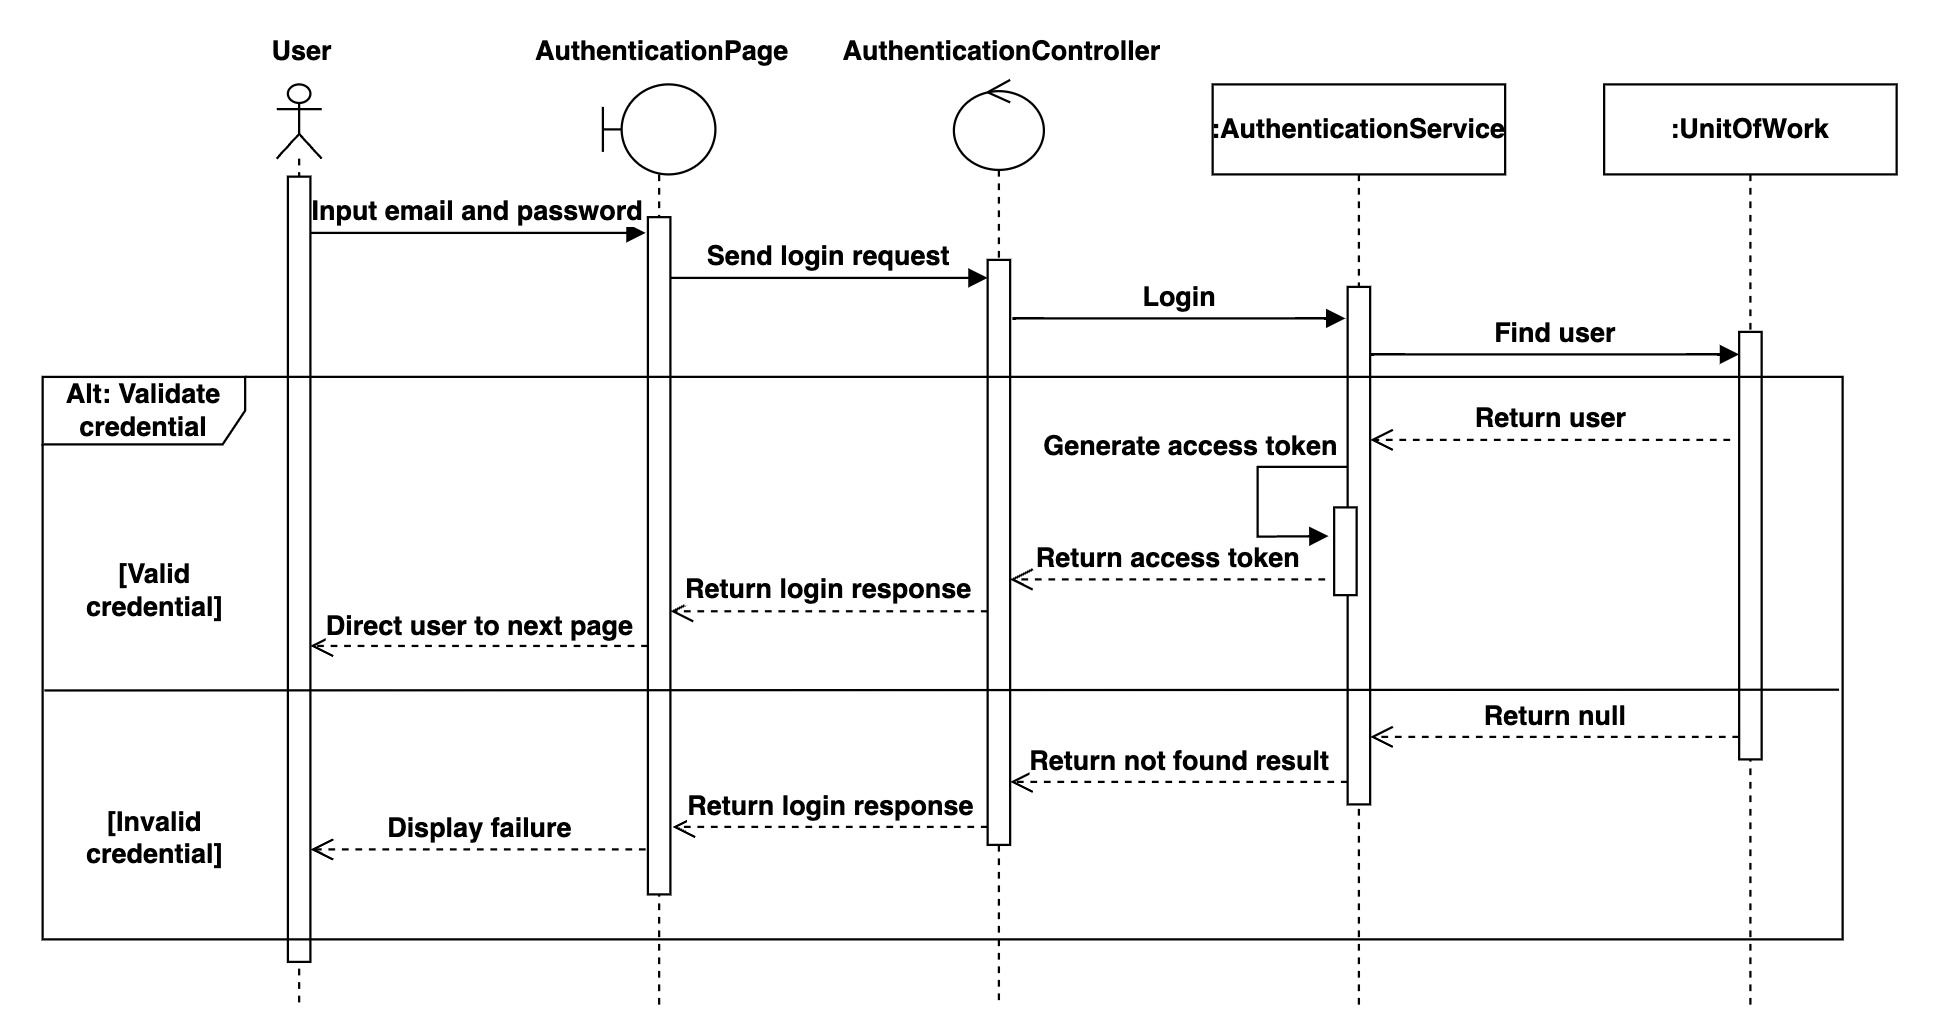
\includegraphics[width=0.9\textwidth]{Figures/login_seq.png}
  \caption{Login sequence diagram}
  \label{fig:login-seq}
\end{figure}
\clearpage
\subsubsection{Login with a Google account}

\begin{figure}[H]
  \centering
  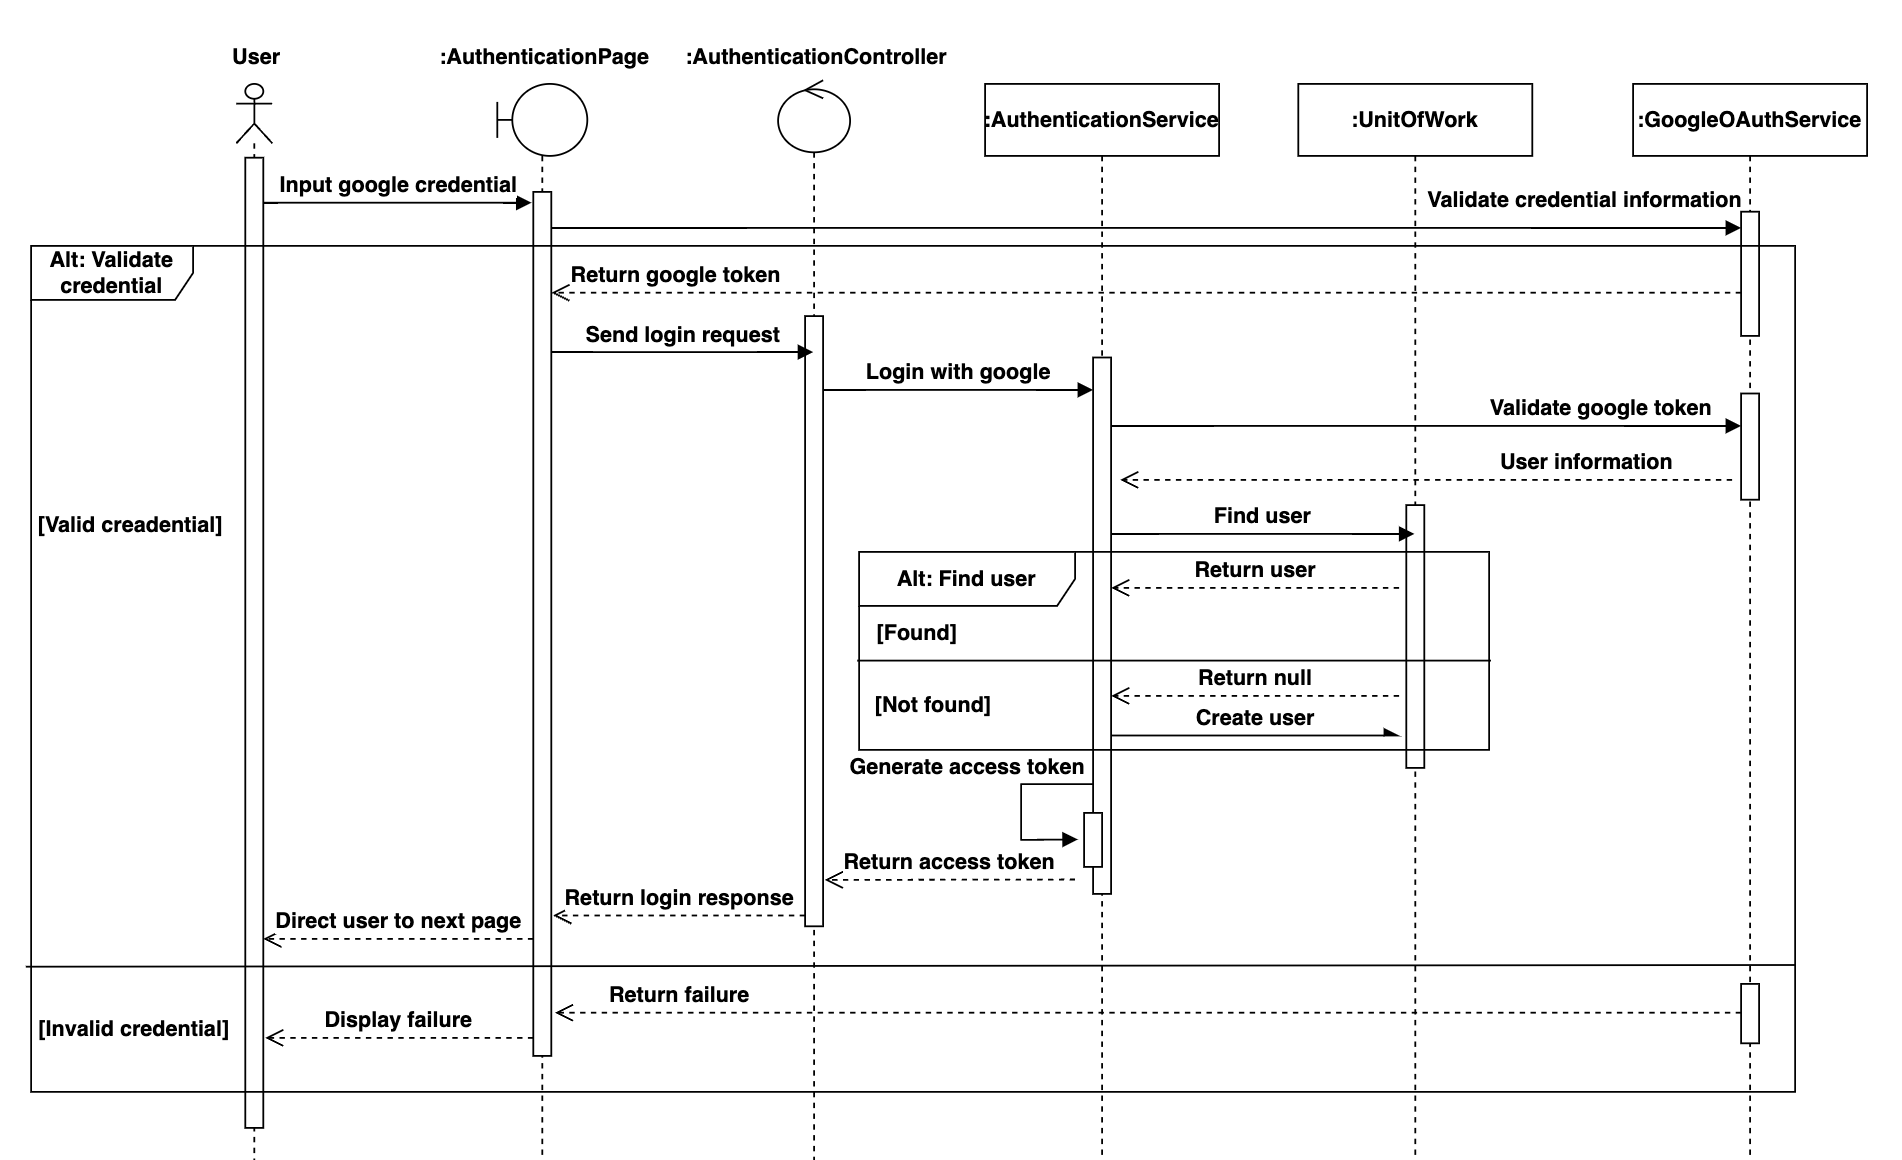
\includegraphics[width=0.9\textwidth]{Figures/login_gg_seq.png}
  \caption{Login with a Google account sequence diagram}
  \label{fig:login-google-seq}
\end{figure}

\subsubsection{Update to Organization account}

\begin{figure}[H]
  \centering
  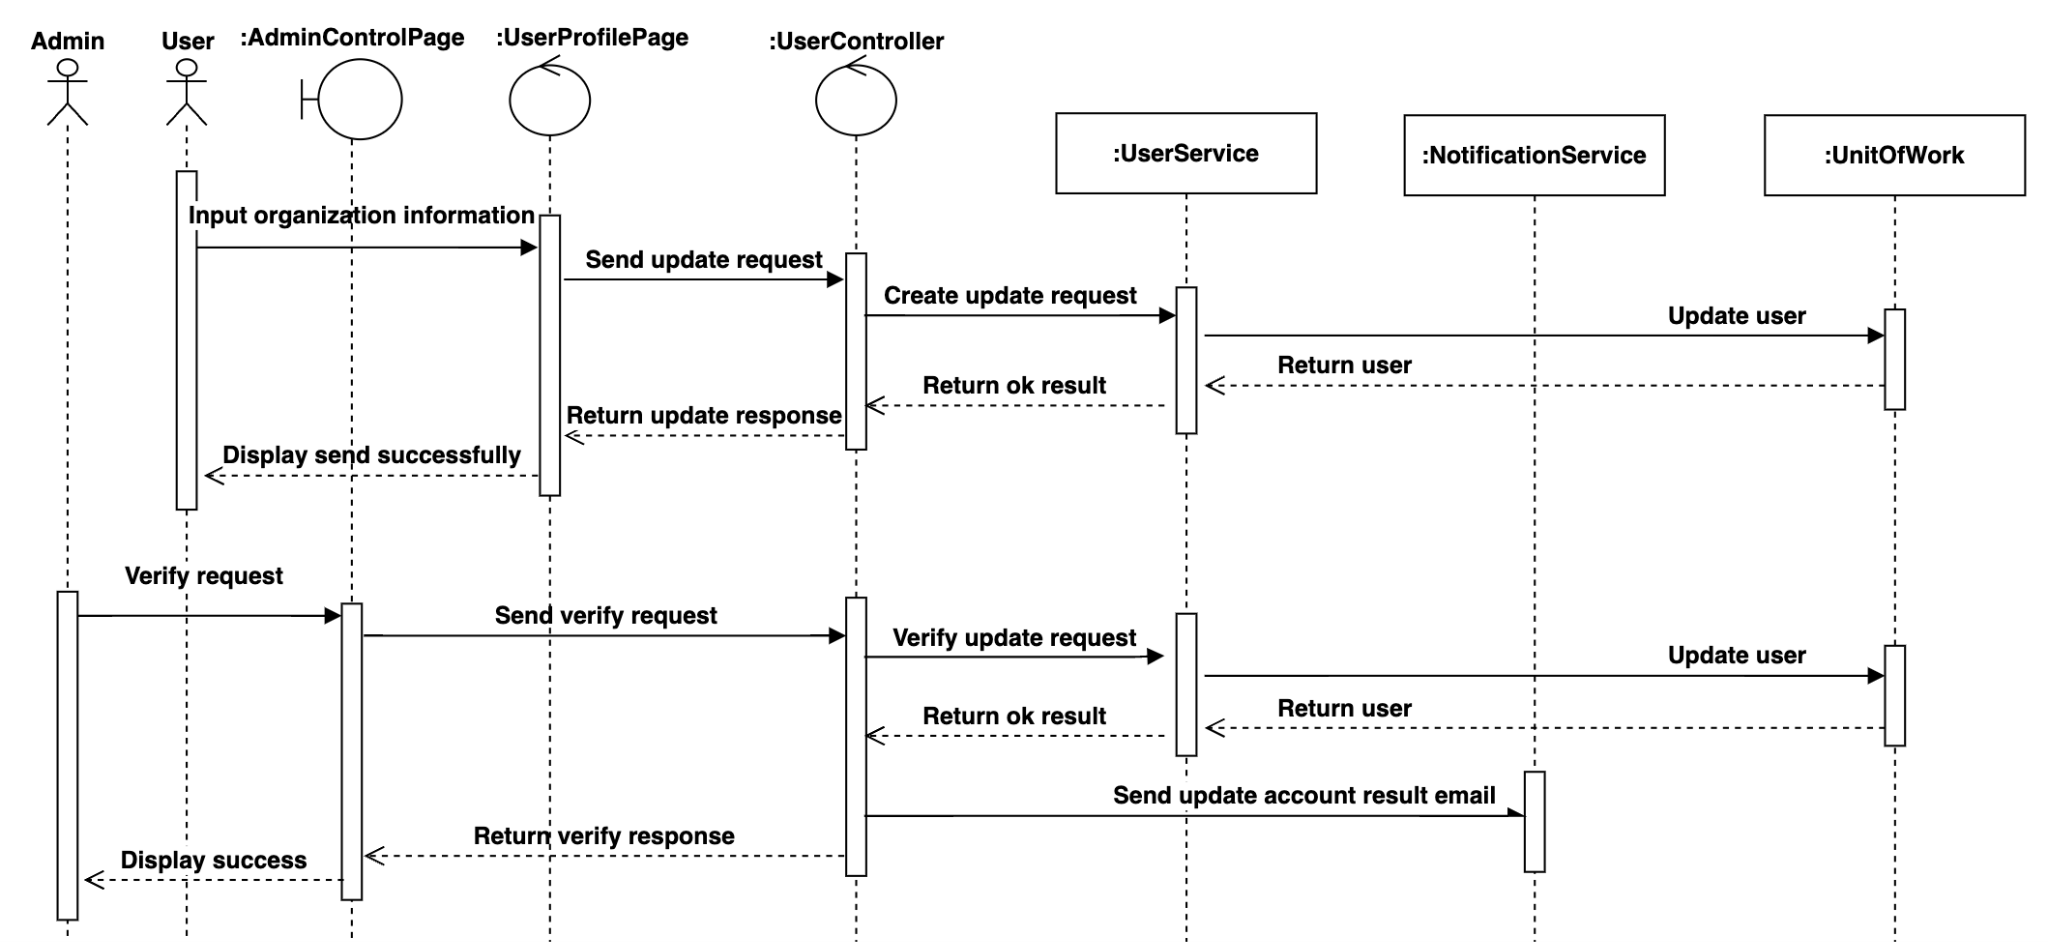
\includegraphics[width=0.9\textwidth]{Figures/update_org_seq.png}
  \caption{Update to Organization account sequence diagram}
  \label{fig:update-org-seq}
\end{figure}

\subsubsection{Manage pet profile}

\begin{figure}[H]
  \centering
  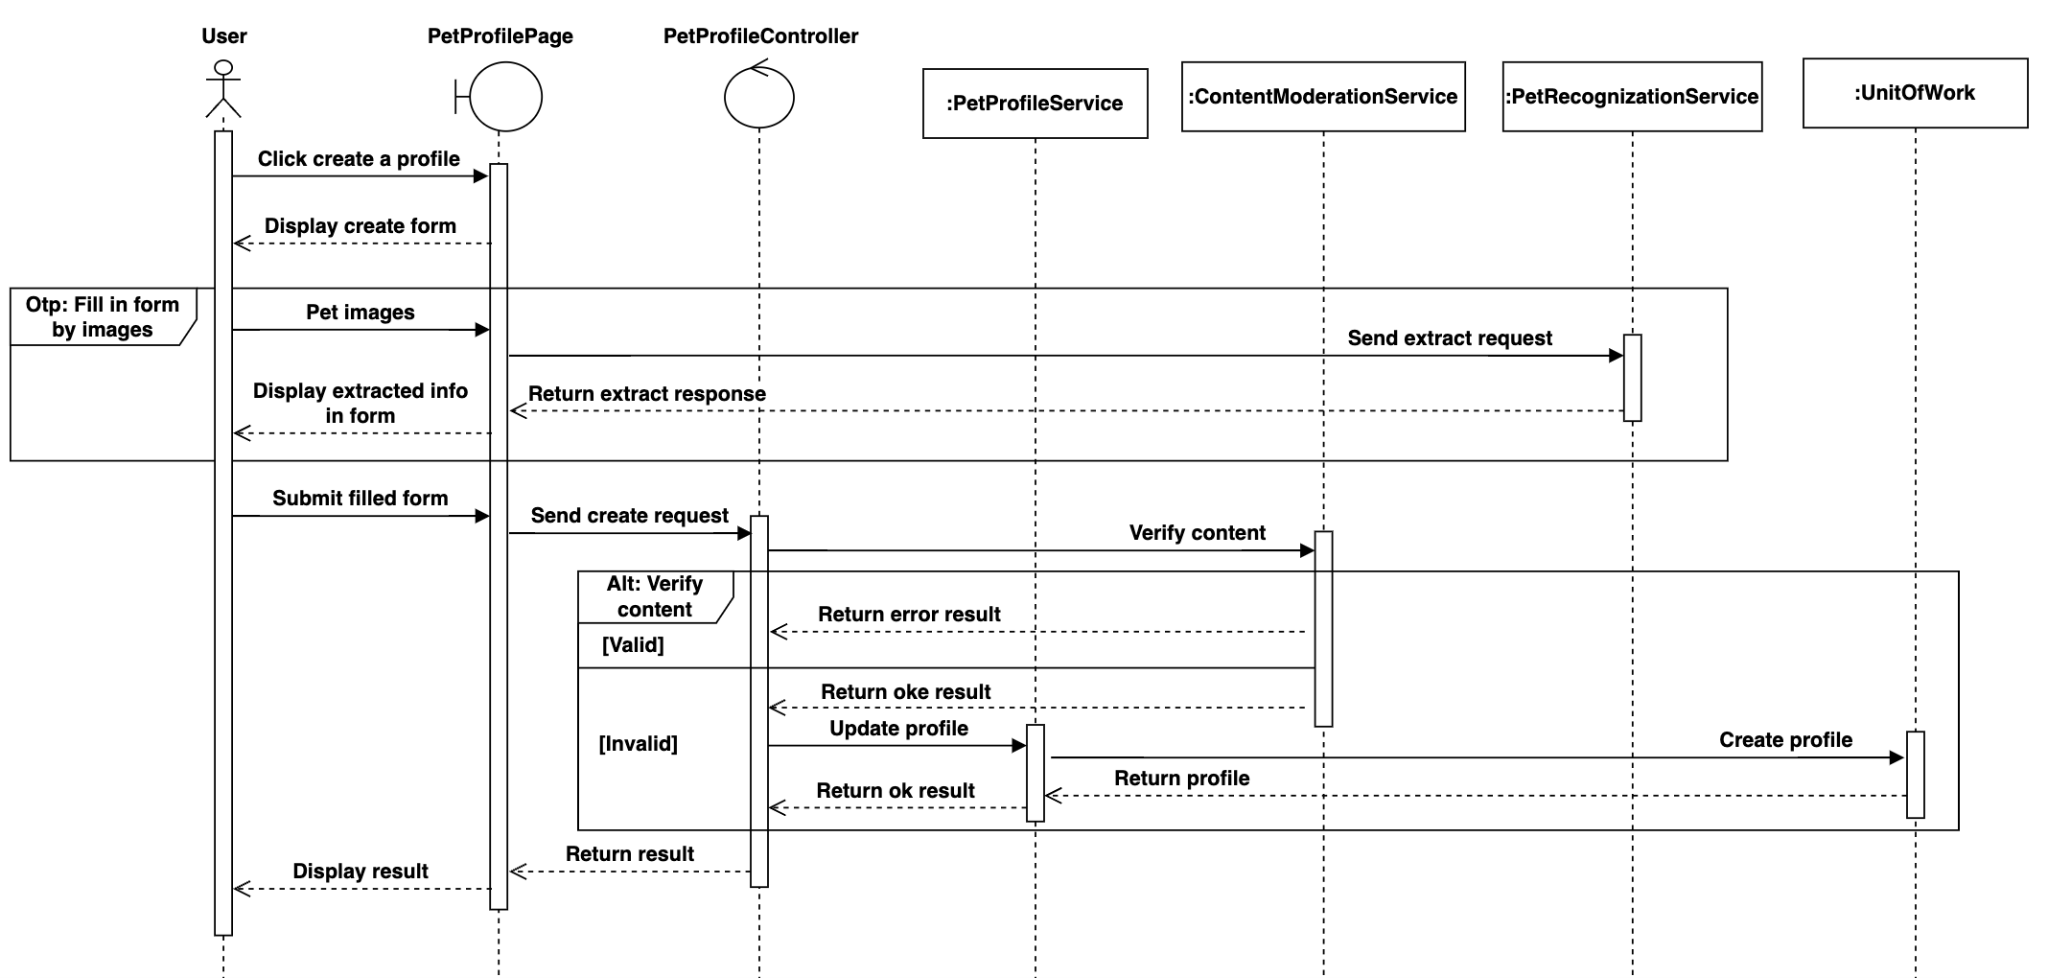
\includegraphics[angle=-90,width=0.7\textwidth]{Figures/manage_pet_seq.png}
  \caption{Create pet profile sequence diagram}
  \label{fig:manage-pet-seq}
\end{figure}
\clearpage
\begin{figure}[H]
  \centering
  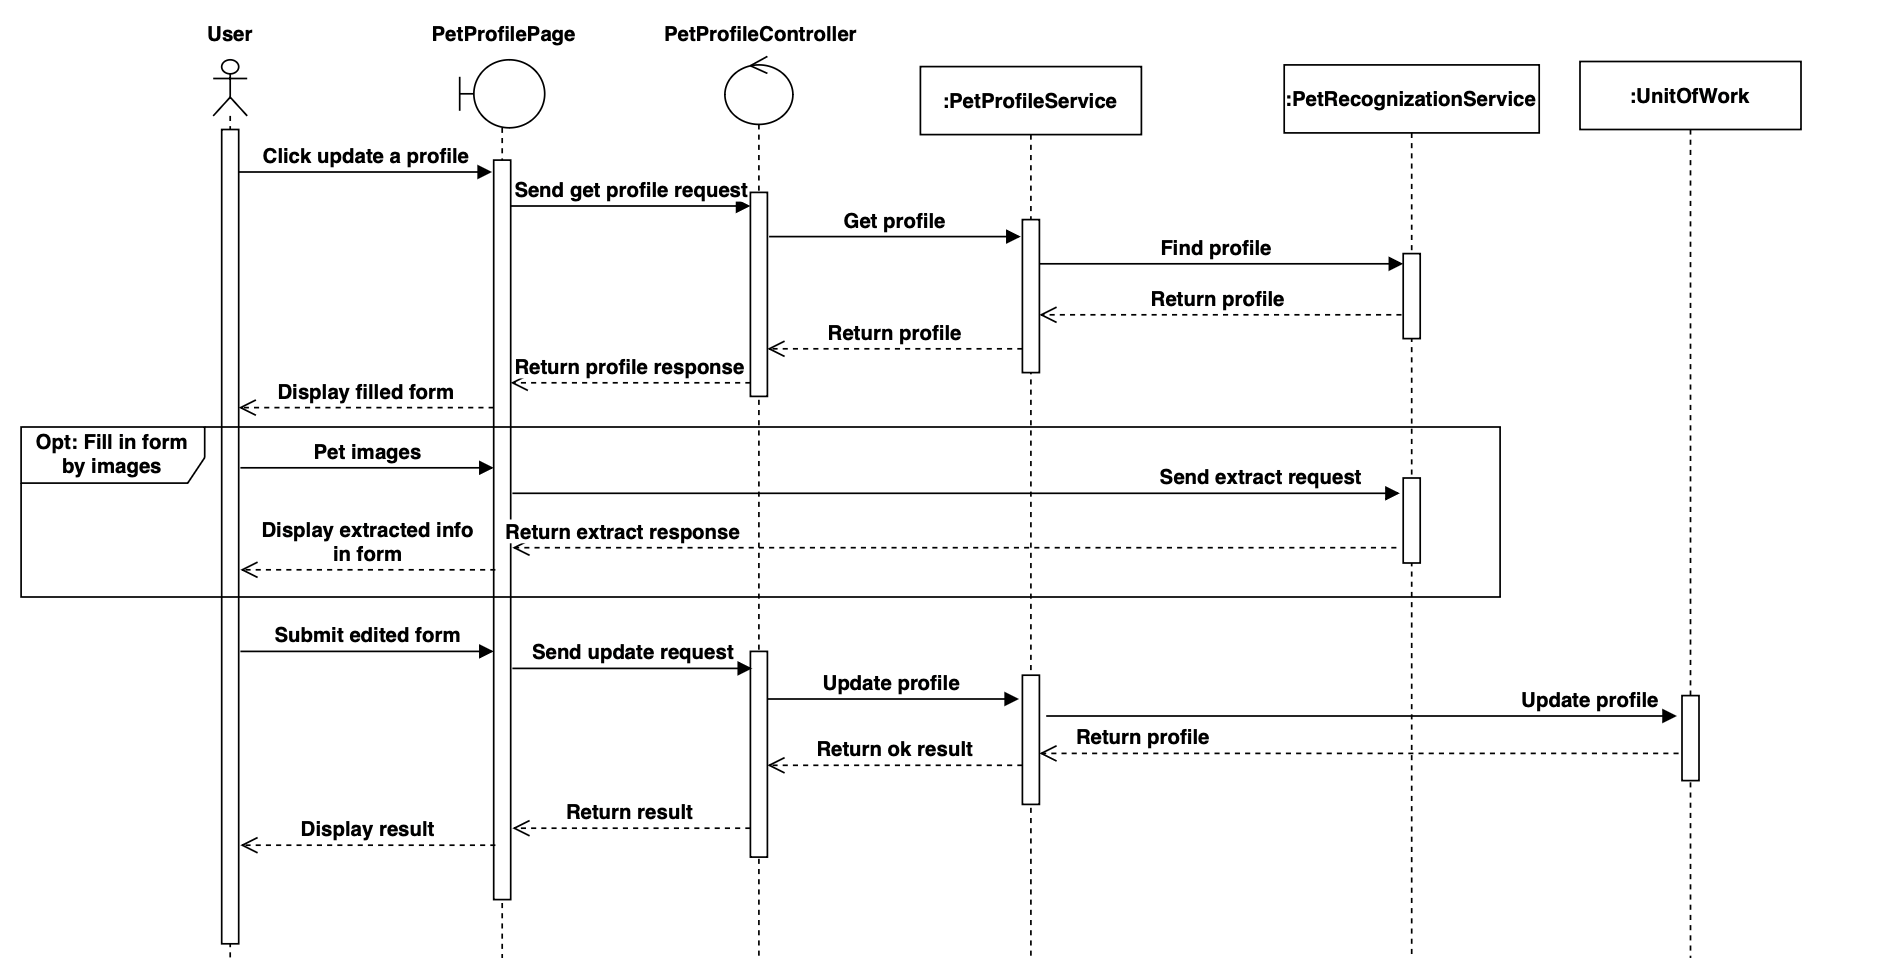
\includegraphics[angle=-90,width=0.7\textwidth]{Figures/update_pet_profile_seq.png}
  \caption{Update pet profile sequence diagram}
  \label{fig:access-pet-seq}
\end{figure}
\clearpage

\subsubsection{Manage blogs}

\begin{figure}[H]
  \centering
  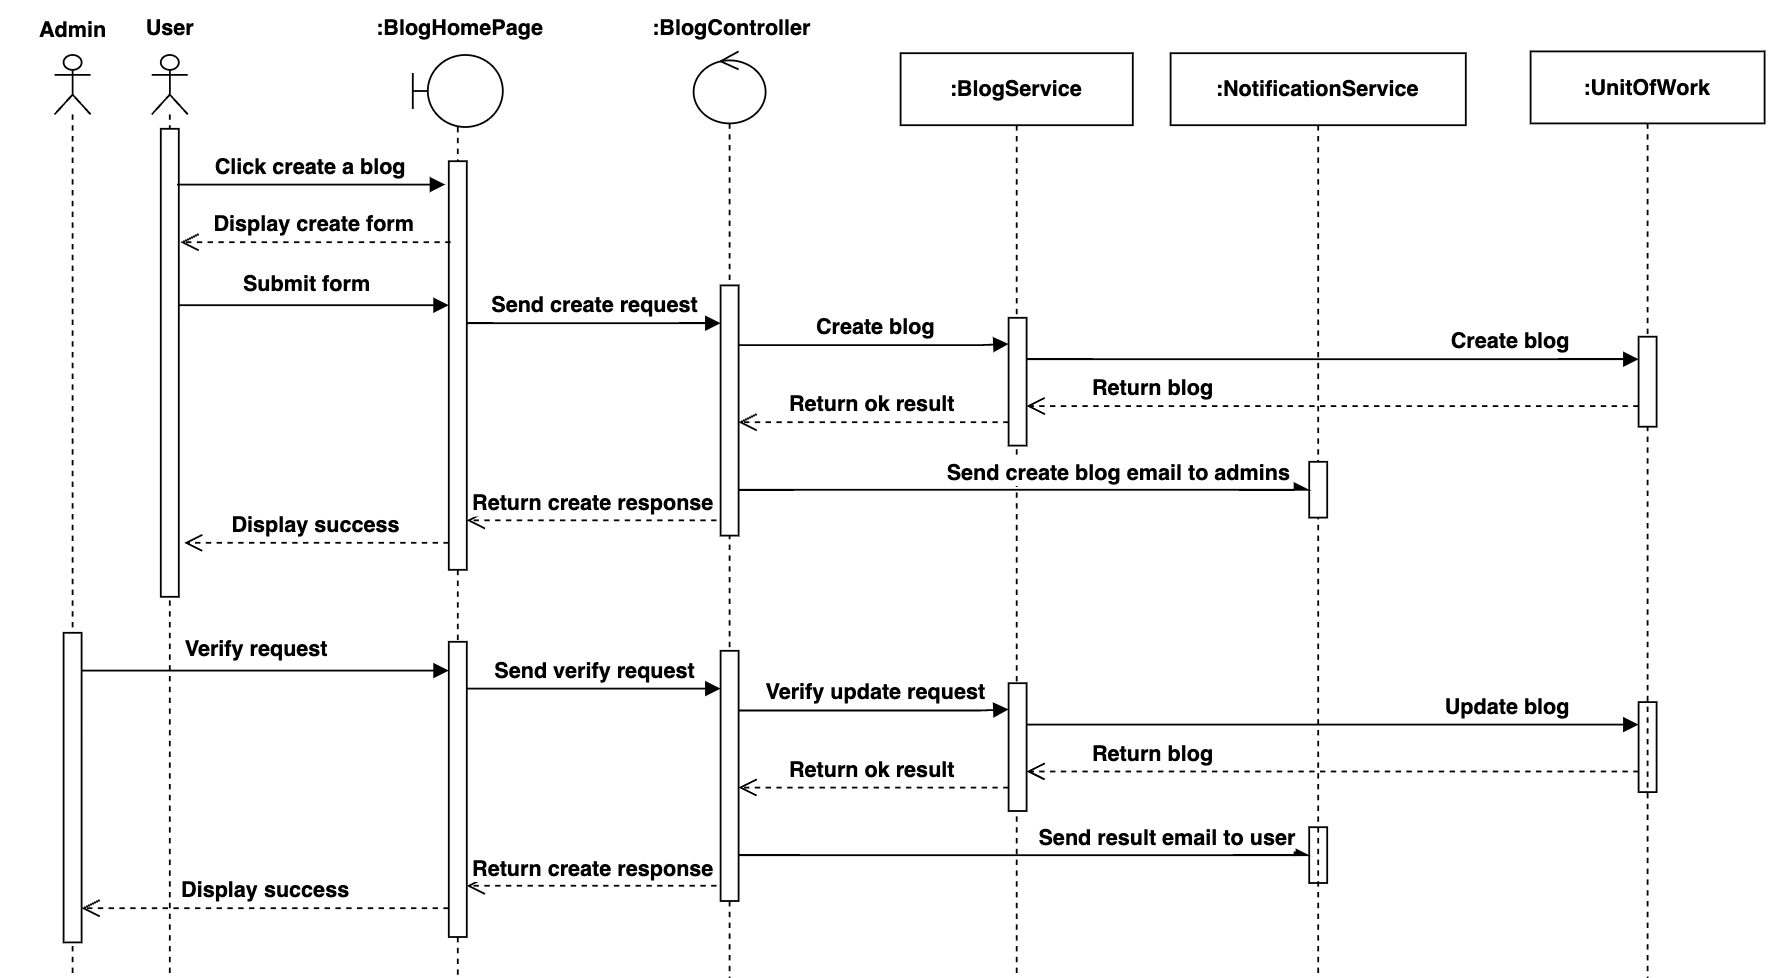
\includegraphics[width=0.9\textwidth]{Figures/manage_blog_seq.png}
  \caption{Create blogs sequence diagram}
  \label{fig:manage-blog-seq}
\end{figure}

\begin{figure}[H]
  \centering
  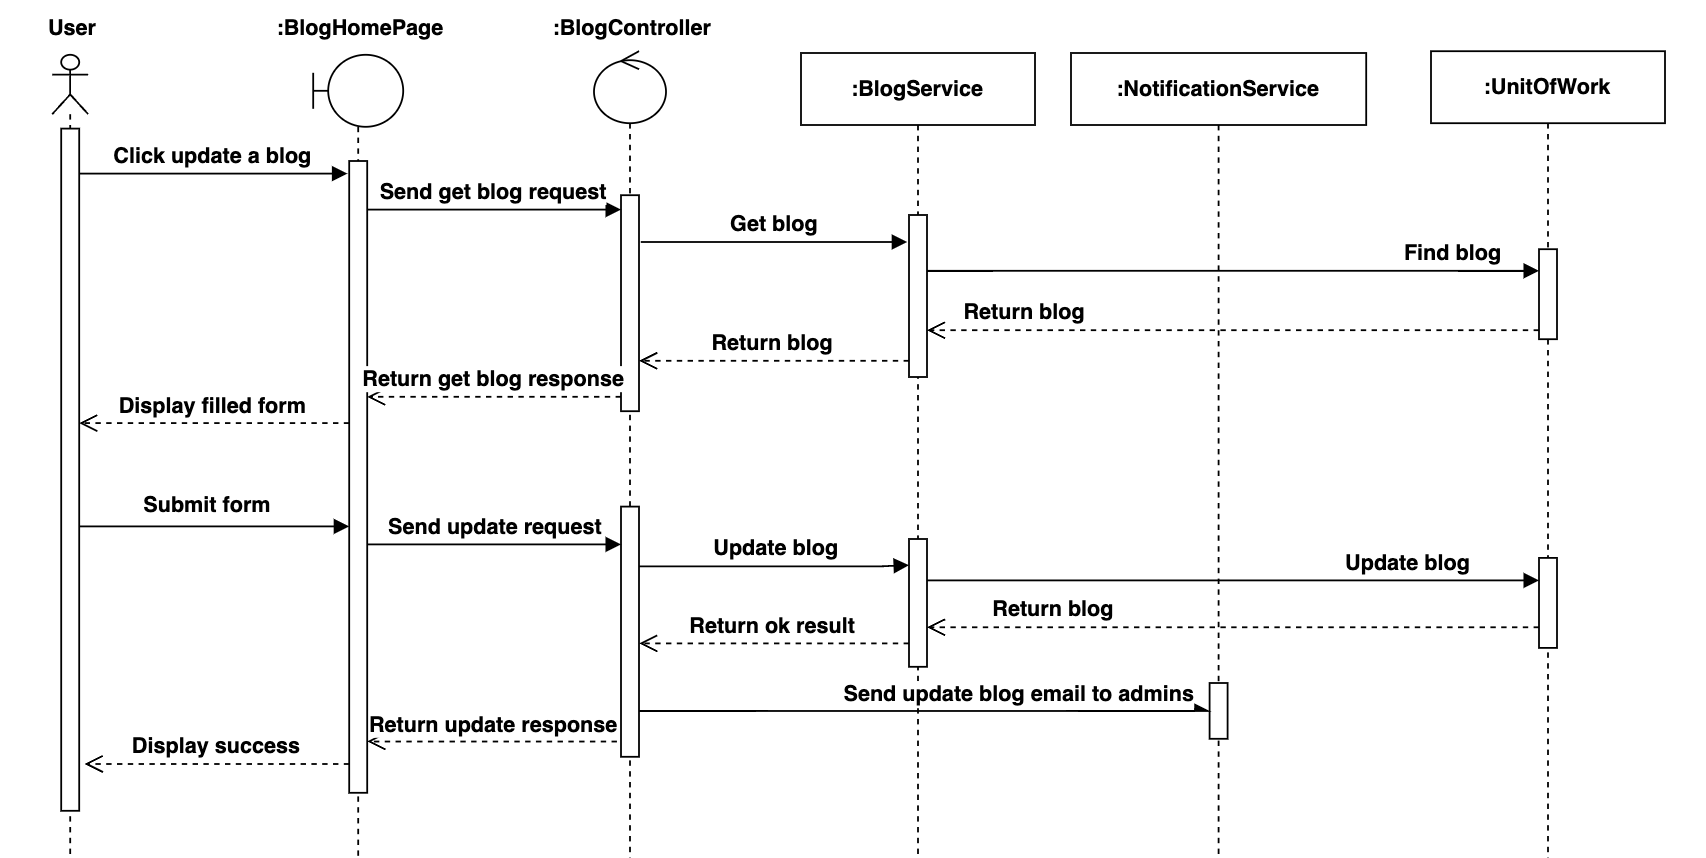
\includegraphics[width=0.9\textwidth]{Figures/update_blog_seq.png}
  \caption{Update blogs sequence diagram}
  \label{fig:update-blog-seq}
\end{figure}
\clearpage
\subsubsection{Make payment}

\begin{figure}[H]
  \centering
  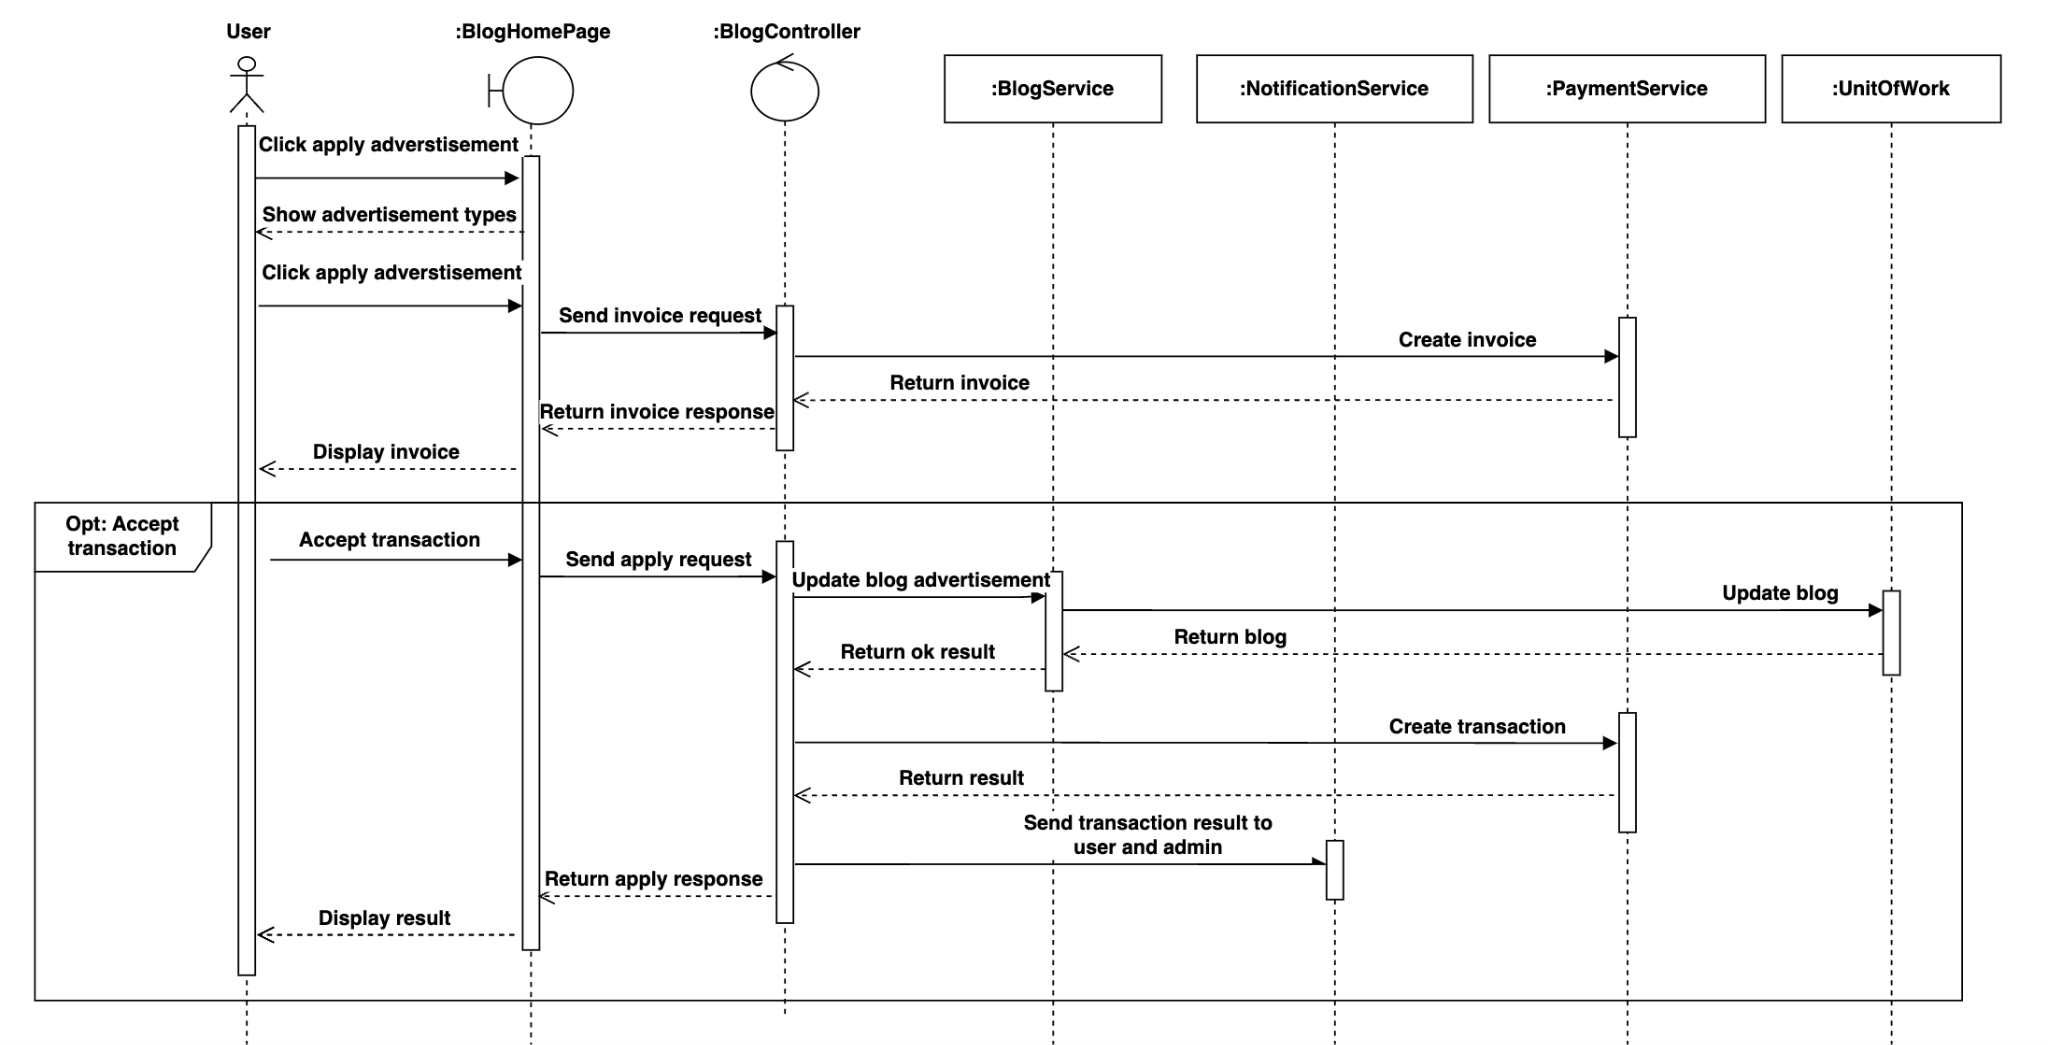
\includegraphics[width=0.9\textwidth]{Figures/payment_seq.png}
  \caption{Make payment sequence diagram}
  \label{fig:make-payment-seq}
\end{figure}


